\documentclass{article}
\usepackage{graphicx}
\usepackage{epstopdf}
\usepackage{floatrow}
\usepackage{chngcntr}
\counterwithin{table}{section}
\usepackage{amsmath}
\usepackage{textcomp}
\usepackage{hyperref}
\usepackage{mhchem}
\hypersetup{
   		colorlinks,
    	citecolor=black,
    	filecolor=black,
    	linkcolor=black,
    	urlcolor=black
	}
\numberwithin{figure}{section}
\numberwithin{equation}{section}
\oddsidemargin=.15in
\evensidemargin=.15in
\textwidth=6in
\topmargin=-.5in
\textheight=9in
\parindent=0in

	\begin{document}
	\author{}
	\title{Perry's recipes}
	\date{}
	\maketitle
	\tableofcontents
	\underline{\hspace{6in}} \\ \\
	\pagenumbering{arabic}

%%%%%%%%%%%%%%%%%%%%%%%%%%%%%%%%%%%%%%%%%%%%%%%%%%%%%%%%%%%%%%%%%%%%

\pagebreak
\section{Breakfast}

\pagebreak
\subsection{Buckwheat Pancakes}
Joy of Cooking\\
Makes about 18 4-inch pancakes. Note, a half recipe is almost too much for two people.\\

{\bf Ingredients}\\
1 cup buckwheat flour\\
1 cup all-purpose flour\\
2 tablespoons sugar\\
1 teaspoon baking soda\\
1 teaspoon salt\\
2 cups buttermilk\\
1/4 cup (1/2 stick) butter, melted\\
2 egg yolks\\
2 egg whites\\

{\bf Instructions}\\
\begin{enumerate}
\item Whisk dry ingredients together in large bowl.
\item Mix wet ingredients in a separate bowl. Pour wet ingredients over dry ingredients and combine with a few quick strokes of the whisk, leaving the batter slightly lumpy.
\item Whish the egg whites until stiff but not dry. This works well with an electric mixer. Fold into batter until just blended.
\end{enumerate}

Buttermilk substitute: for 1 cup buttermilk, add 1 tbs lemon juice or white vinegar to a cup measure and fill the rest with milk.


\pagebreak
\subsection{Popovers}
{\bf Ingredients}\\
1 cup flour\\
0.5 tsp salt\\
1 tsp sugar (optional)\\
2 tbs unsalted butter, melted\\
1 cup milk\\
3 large eggs\\

{\bf Instructions}\\
Makes about 8 popovers
\begin{enumerate}
\item Set out popover/muffin tins - silicone (set on a cookie sheet) are particularly good, don't require grease. Otherwise grease tins.
\item Make batter at least 2 hours before baking, or the night before, or up to two days in advance. Before using, bring to room temperature and stir again.
\item Place ingredients in a blender and zap. Scrape down sides and blend again. Can leave in blender until ready to bake.
\item Adjust oven rack to center-low position and heat to 375. If using metal or glass tins, place them (empty) in oven while heating.
\item Spray (metal or glass) tins and pan rim.
\item Fill each cup cup nearly full with batter and bake until popovers are light brown, 45-50 minutes, depending on size.  DO NOT OPEN OVEN DURING BAKING.
\end{enumerate}

{\bf Variations}\\
Savory popovers: add 1/3 cup chopped chives, or some fresh thyme and 1/4 tsp pepper or some lemon zest. Add parsley and Parmesan. Add rosemary and pepper. Add 1/2 cup of grated cheese.

\pagebreak
\subsection{Banana Bread}
{\bf Ingredients}\\
1 1/3 cups flour (part wheat germ)\\
1 teaspoon baking soda\\
1/4 teaspoon baking powder\\
1/4 teaspoon salt\\
pinch nutmeg\\
6 tablespoons butter (3/4 stick)\\
1/2 cup sugar\\
1 teaspoon lemon juice\\
1 1/4 cups ripe banana, mashed\\
2 large eggs\\

{\bf Instructions}
\begin{enumerate}
\item Grease 1 loaf pan pan, then flour lightly and set aside.  Mash bananas into a measuring cup to measure quantity.

\item Sift dry ingredients by measuring into the Cuisinart bowl and pulsing briefly.  Remove to a mixing bowl.

\item If including nuts, chop at this time in Cuisinart; set aside.

\item Cut butter into pieces and put into empty, Cuisinart bowl along with sugar and lemon juice.  Process well and scrape down sides.

\item Measure banana and add to butter. Blend.

\item Add eggs and blend. Scrape sides.  Heat oven to 350 and set rack in lower third.

\item Pour butter into flour and stir only until well mixed. (Add nuts and/or chocolate chips if desired.)  Pour into loaf pan and bake for 1 - 1.25 hr.  Test with a knife in the center to see if done.  Let sit 10 minutes in the pan, then remove to a cooking rack.

\end{enumerate}

VARIATIONS:\\
Add 1 cup walnuts, add nuts after banana and pulse briefly.\\

CHOCOLATE CHIPS:  For a dessert version, increase sugar to ¾ cup and change nuts to pecans, and stir in 1 cup chocolate chips at the end.\\

BANANA COCONUT:  Add 1/2 tsp almond extract and 1 cup toasted, flaked coconut.\\

If banana is ripe before you are ready to cook, freeze the pulp, then defrost to use.

\pagebreak
\subsection{Crepes}
{\bf Ingredients}\\
3 large eggs\\
1 cup whole milk*\\
6 tablespoons water\\
1 cup flour\\
1/2 teaspoon salt\\
2 tablespoons canola (or part melted butter)\\

*If using low-fat milk, replace both whole milk and water with low-fat milk.\\

{\bf Instructions}
\begin{enumerate}
\item Throw all the above ingredients in a blender (or food processor, or mix well by hand).  Transfer batter to a covered container and store in the refrigerator at least 1/2 hour and up to 48 hours.
\item Gently stir up batter, it should be slightly thicker than heavy cream.  Heat a 7-8 in crepe pan or small heavy skillet over medium-high heat.  Brush the bottom with melted butter or vegetable oil.  When pan is hot, pour in 2 1/2 tablespoons batter, swirl pan to coat evenly.  Cook 30 seconds to 1 minute until mottled brown on the bottom, loosen the crepe and flip.  Cook another 30 seconds on the other side.  For a 9 - 10in skillet use 1/4 cup batter.
\item If not eaten right away, crepes can be double-wrapped in plastic and refrigerated up to 3 days or frozen up to 2 months.  To freeze, stack up 8 crepes, wrap in plastic wrap, then in foil, for several weeks.  To thaw, switch them from the freezer, directly to the refrigerator.  This will take about 3 hours.
\end{enumerate}

\pagebreak
\subsection{Oatmeal Muffins}
Makes 10-12 muffins\\

{\bf Ingredients}\\
1 cup rolled oats\\
1 cup buttermilk\\
1 cup flour\\
1/2 teaspoon salt\\
1/2 teaspoon soda\\
1 1/2 teaspoons baking powder\\
0.4 cup vegetable oil\\
1/3 cup brown sugar\\
1 egg, beaten\\

{\bf Instructions}
\begin{enumerate}
\item Combine oats and buttermilk in a large mixing bowl and soak for 30 minutes or longer.
\item Sift flour with salt, soda, and baking powder, set aside.  
\item Add vegetable oil, brown sugar, and beaten egg to oatmeal mixture and blend thoroughly.
\item Stir in dry ingredients and mix only long enough to moisten.
\item Spoon into sprayed muffin tins.
\item Bake at 350 degrees for 22-25 minutes or until lightly brown. (Muffins do  not rise very high)
\end{enumerate}

NIGHT BEFORE: Combine together in a large bowl: oats, buttermilk, oil, brown sugar, and beaten egg.  Cover and refrigerate.  Prepare sifted dry ingredients and muffin tins.  Bring cold batter to room temp before mixing.

VARIATIONS: 
\begin{itemize}
\item Substitute buttermilk with yoghurt (slightly diluted with milk or water).
\item To make (24-28) mini-muffins, reduce cooking time to 20 minutes.
\end{itemize}

\pagebreak
\subsection{Granola}
{\bf Ingredients}\\
2 pounds oats\\
2 pounds nuts, seeds, etc. (e.g. shredded coconut, sunflower seeds, pumpkin seeds, chia seeds, flax seeds, almonds, walnuts, pecans, cashews)\\
1/2 cup vegetable oil\\
1/2 cup honey\\
Dried fruit\\

{\bf Instructions}
\begin{enumerate}
\item Combine ingredients. Spread on two baking sheets (silpats help if you have them).
\item Bake at 275 F for 40-45 minutes stirring once mid-way.
\item Add dried fruit. NB: storing granola with dried fruit can make it less crisp. May want to add dried fruit only when serving.
\end{enumerate}

NOTES: Freezes well.


\pagebreak
\section{Bready things}

\pagebreak
\subsection{Classic Pizza Dough}
{\bf Ingredients}\\
4-4.25 cups bread flour\\
2.25 tsp instant yeast\\
1.5 tsp salt\\
2 tbs EVOO\\
1.5 cups water, heated to 110 degrees\\

{\bf Instructions}
\begin{enumerate}
\item Pulse 4 cups flour, yeast, and salt in food processor until combined.  With food processor running, slowly add oil, then water; process until rough ball forms, 30 to 40 seconds.  Let dough rest 2 minutes, the process 30 seconds more.  (If, after 30 seconds dough is sticky and clings to blade, add remaining 0.25 cup flour 1 tbs at a time as needed.)
\item Transfer dough to lightly floured counter and knead by hand until smooth, round ball.  Place dough in a large, lightly greased bowl; cover tightly with plastic and let rise at room temperature until doubled (1 to 1.5 hours).
\end{enumerate}


\pagebreak
\subsection{NY Times no-knead bread}
{\bf Ingredients}\\
3 cups all-purpose flour or bread flour, more for dusting\\
0.25 tsp instant yeast\\
1.25 tsp salt\\
Cornmeal or wheat bran as needed\\

{\bf Instructions}
\begin{enumerate}
\item In a large bowl combine flour, yeast and salt.  Add 1 5/8 cups water, and stir until blended; dough will be shaggy and sticky.  Cover bowl with plastic wrap.  Let dough rest at least 12 hours, preferably about 18, at warm room temperature, about 70 degrees.
\item Dough is ready when its surface is dotted with bubbles.  Lightly flour a work surface and place dough on it; sprinkle it with a little more flour and fold it over on itself once or twice.  Cover loosely with plastic wrap and let rest about 15 minutes.
\item Using just enough flour to keep dough from sticking to work surface or to your fingers, gently and quickly shape dough into a ball. Generously coat a cotton towel (not terry cloth) with flour, wheat bran or cornmeal; put dough seam side down on towel and dust with more flour, bran or cornmeal. Cover with another cotton towel and let rise for about 2 hours. When it is ready, dough will be more than double in size and will not readily spring back when poked with a finger.
\item At least a half-hour before dough is ready, heat oven to 450 degrees. Put a 6- to 8-quart heavy covered pot (cast iron, enamel, Pyrex or ceramic) in oven as it heats. When dough is ready, carefully remove pot from oven. Slide your hand under towel and turn dough over into pot, seam side up; it may look like a mess, but that is O.K. Shake pan once or twice if dough is unevenly distributed; it will straighten out as it bakes. Cover with lid and bake 30 minutes, then remove lid and bake another 15 to 30 minutes, until loaf is beautifully browned. Cool on a rack.
\end{enumerate}

NOTE: Consider putting parchment paper at the bottom of the pot to prevent the bread from sticking. The dough should not stick if the pot is sufficiently hot.


\pagebreak
\subsection{NY Times no-knead wheat bread}
{\bf Ingredients}\\
2 2/3 cups bread flour\\
1 1/3 cups wheat flour\\
2 tsp salt\\
1/2 tsp yeast\\
2 cups water\\

{\bf Instructions}
\begin{enumerate}
\item Mix ingredients well in a large bowl. Cover with plastic wrap (tip: wetting the outside rim of the bowl will help the plastic wrap stick). Let rise for $\sim$12 hours.

\item Gently remove dough onto relatively heavily-floured surface, and fold dough 3 times. Try to minimize the amount you manipulate the dough. Place on a floured cloth and cover loosely with plastic wrap. Let rise for $\sim$2 hours.

\item Preheat oven to 500-550 $^{\circ}$F, and place a dutch oven (with lid off but in oven) in the oven to also preheat. Once pre-heated, gently place dough in hot dutch oven, cover with lid, and bake for 30 minutes. Remove lid, and bake an additional 15 minutes. Unless eating immediately, allow sufficient time to cool before cutting.

\end{enumerate}


\pagebreak
\subsection{NY Times speedy no-knead bread}
{\bf Ingredients}\\
3 cups bread flour\\
1 packet (1/4 ounce; 2.25 tsp) instant yeast\\
1.5 tsp salt\\
Oil as needed\\

{\bf Instructions}
\begin{enumerate}

\item Combine flour, yeast and salt in a large bowl. Add 1 1/2 cups water and stir until blended; dough will be shaggy. Cover bowl with plastic wrap. Let dough rest about 4 hours at warm room temperature, about 70 degrees.

\item Lightly oil a work surface and place dough on it; fold it over on itself once or twice. Cover loosely with plastic wrap and let rest 30 minutes more.

\item At least a half-hour before dough is ready, heat oven to 450 degrees. Put a 6-to-8-quart heavy covered pot (cast iron, enamel, Pyrex or ceramic) in oven as it heats. When dough is ready, carefully remove pot from oven. Slide your hand under dough and put it into pot, seam side up. Shake pan once or twice if dough is unevenly distributed; it will straighten out as it bakes.

\item Cover with lid and bake 30 minutes, then remove lid and bake another 15 to 30 minutes, until loaf is beautifully browned. Cool on a rack.
\end{enumerate}

NOTE: Consider putting parchment paper at the bottom of the pot to prevent the bread from sticking. The dough should not stick if the pot is sufficiently hot.


\pagebreak
\subsection{Southern-Style Cornbread}
{\bf Ingredients}\\
4 teaspoons bacon drippings or 1 tablespoon melted unsalted butter plus 1 teaspoon vegetable oil\\
1 cup (5 ounces) stone-ground cornmeal\\
2 teaspoons granulated sugar\\
1 teaspoon baking powder\\
0.25 teaspoon baking soda\\
0.5 teaspoon salt\\
1/3 cup boiling water\\
0.75 cup buttermilk\\
1 large egg, lightly beaten\\

{\bf Instructions}
\begin{enumerate}
\item Adjust oven rack to lower middle position and heat to 450 degrees.  Add bacon drippings to 8-inch cast-iron skillet and place skillet in preheating oven.

\item Place 1/3 cup cornmeal in medium bowl and set aside.  Mix remaining 2/3 cup cornmeal, sugar, baking powder, baking soda, and salt in small bowl; set aside.
	
\item Pour boiling water over reserved 1/3 cup cornmeal and stir to make stiff mush.  Gradually whisk in buttermilk, breaking up lumps until smooth.  Whisk in egg.  When oven is up to temperature and skillet very hot, stir dry ingredients into mush mixture until just moistened.  Carefully remove skillet from oven.  Pour hot bacon fat from skillet into batter and stir to incorporate, then quickly pour batter into heated skillet.  Bake until golden brown, about 20 minutes.  Remove from oven and immediately turn cornbread onto wire rack; let cool for 5 minutes and serve.
\end{enumerate}

\pagebreak
\subsection{Flying Biscuits}
{\bf Ingredients}\\
3 cups all-purpose flour\\
1 tbs plus 1.5 tsp baking powder\\
0.75 tsp salt\\
2 tbs plus 1.5 tsp sugar\\
6 tbs unsalted butter\\
2/3 cup heavy cream\\
2/3 cup half and half (plus 1 tbs for brushing the top of the biscuits)\\

{\bf Instructions}
\begin{enumerate}
\item Preheat oven to 350$^\circ$F. Line a sheet pan with parchment paper.

\item Place flour, baking powder, salt, and sugar in a large mixing bowl. Cut butter into 1/2 tablespoon-sized-bits and add to the flour. Using your fingertips or a pastry cutter, work the butter into the flour mixture until it resembles coarse meal. Make a well in the center of the flour and pour in all the heavy cream and the half and half.

\item Stir the dry ingredients into the cream and mix with a wooden spoon until dough just begins to come together into a ball. Turn dough onto a lightly floured surface and knead 2 or 3 times to form a cohesive mass. Do not overwork the dough.

\item Using a rolling pin, roll the dough to a .5 inch thickness.  Cut out biscuits using a ~2 inch circular thing.

\item Place the biscuits on the prepared sheet pan, leaving about 1/4 inch between them.

\item Brush the tops of the biscuits with 1 tablespoon of half and half.

\item Bake for 20 minutes. Biscuits will be barely browned on top and flaky in the center when done. (Don’t overcook them – otherwise they get hard).
\end{enumerate}


\pagebreak
\subsection{Pita Bread}
Makes 8 pitas\\

{\bf Ingredients}\\
3 cups flour\\
1 1/2 teaspoons salt\\
1 Tablespoon sugar or honey\\
1 packet yeast (or, if from bulk, 2 teaspoons yeast)\\
1 1/4 to 1.5 cups water, roughly at room temperature\\
2 tablespoons olive oil, vegetable oil, butter, or shortening\\

{\bf Instructions}
\begin{enumerate}
\item Mix yeast with flour, salt, and sugar.  Add olive oil and 1 1/4 cup water and stir.  All of the ingredients should form a ball. If some of the flour will not stick to the ball, add more water (I had to add an extra 1/4 cup). 

\item Knead dough approximately 10 minutes (or until your hands get tired). If you are using an electric mixer, mix it at low speed for 10 minutes.  Form dough into a ball and place it in lightly oiled bowl.  Cover bowl with plastic and let rise until doubled (~90 min).

\item When doubled, punch down divide it into 8 pieces. Roll each piece into a ball, cover with a damp kitchen towel, and let rest for 20 minutes.

\item While the dough is resting, preheat the oven to 400 degrees and insert pizza stone. If you do not have a baking stone, turn a cookie sheet upside down and place it on the middle rack of the oven while you are preheating the oven.

\item Roll, stretch, and generally flatten dough on lightly floured surface. Should be between 1/8 and 1/4 inch thick. If the dough does not stretch sufficiently you can cover it with the damp towel and let it rest 5 to 10 minutes before trying again.

\item They should be baked through and puffy after 3 minutes. If you want your pitas to be crispy and brown you can bake them for an additional 3 to 5 minutes, but it isn't necessary (in the batch pictured here I removed them at 3 minutes).
\end{enumerate}

%%%%%%%%%%%%%%%%%%%%%%%%%%%%%%%%%%%%%%%%%%%%%%%%%%%%%%%%%%%%%%%%%%%%
\pagebreak
\section{Soups}

\pagebreak
\subsection{Potage Parmentier (leek and potato soup)}
Lorraine Spector (possibly originally from Cooks Illustrated)\\

{\bf Ingredients}\\
1 pound (3 cups) leeks\\
1-2 tablespoons butter\\
1 pound (3 cups) potatoes (Idaho or starchy)\\
6 cups chicken stock, water, or some combination\\
1.5 teaspoons salt (potentially more to taste)\\

OPTIONAL\\
4 tablespoons sour cream or 1.5 oz butter\\
3 tablespoons parsley, chervril, tarragon, or chive garni\\

{\bf Instructions}\\
\begin{enumerate}
\item Slice white and tender green parts of leeks along long axis. Wash, then chop. Sautee in large saucepan with butter.
\item Cut potatoes to 3/4 inch cubes. Add to leeks. Add enough water to cover by 1/2 inch.
\item Bring to boil, partially cover, reduce heat to low, then simmer until tender, about 30-40 minutes.
\item Process vegetables in several batches in a mouli (best), or through a food processer or blender, or press with a potato masher. Additional water or milk can be added if too thick. The soup can be served directly, or returned to saucepan and reheated when ready to serve.
\end{enumerate}


OPTIONAL:  To each bowl, add a spoonful of heavy cream, yogurt or a small pat of softened butter.  Sprinkle with minced parsley or chopped chives.\\

{\bf Variations, or Soupe Du Jour}\\
In the beginning, add chopped carrots or tomatoes. \\
OR, half-way through add diced cauliflower, cucumbers, broccoli, zucchini, or lima beans. \\
OR, 5 minutes before the end of cooking add diced, cooked leftover vegetables.\\
OR, can replace part of water with milk, or add powdered milk.\\
OR, make it creamy by adding 1/2 C heavy cream just before serving.\\
Flavoring - add pepper, marjoram, basil, savory and/or bay leaf\\

CHILLED:  Add a little more salt  and 1/2 C cream before refrigerating, then taste again before serving.\\
OR, add a bunch watercress leaves and stems for last 5 minutes of cooking.  Puree.




\pagebreak
\subsection{Lemony Carrot and Cauliflower Soup}
Melissa Clark, NYT Cooking\\

{\bf Ingredients}\\
1 tablespoon coriander seeds\\
2 tablespoons extra-virgin olive oil, more for serving\\
1 large white onion, peeled and diced (2 cups)\\
2 large garlic cloves, finely chopped\\
5 medium carrots (1 pound), peeled and cut into 1/2-inch pieces (2 cups)\\
1.5 teaspoons kosher salt, more as needed\\
3 tablespoons white miso\\
1 small (or half of a large) head cauliflower, trimmed and cut into florets\\
1/2 teaspoon lemon zest\\
2 tablespoons lemon juice, more to taste\\
Smoky chile powder, for serving\\
Coarse sea salt, for serving\\
Cilantro leaves, for serving\\

{\bf Instructions}
\begin{enumerate}
\item In a large, dry pot over medium heat, toast coriander seeds until fragrant and dark golden-brown, 2 to 3 minutes. Transfer to a mortar and pestle and coarsely crush.
\item Return the pot to medium heat. Add the oil and heat until warm. Stir in onion; cook, stirring occasionally, until soft and lightly colored, 7 to 10 minutes. Stir in garlic and cook 1 minute.
\item Add carrots, crushed coriander, salt and 6 cups water to the pot. Stir in the miso until it dissolves. Bring mixture to a simmer and cook, uncovered, 5 minutes. Stir in cauliflower and cook, covered, over medium-low heat until the vegetables are very tender, about 10 minutes.
\item Remove the soup from the heat. Using an immersion blender, purée the soup until smooth. (Alternatively, you can let soup cool slightly then purée it in batches in a food processor or blender.) If necessary, return the puréed soup to the heat to warm through. Stir in the lemon zest and juice just before serving. Drizzle with oil and sprinkle with chile, sea salt and cilantro leaves.
\end{enumerate}



\pagebreak
\subsection{Roasted Tomato and White Bean Stew}
Colu Henry, NYT Cooking\\

{\bf Ingredients}\\
1/2 cup roughly chopped Italian parsley leaves and tender stems\\
2 tsp lemon zest (from 1 large lemon) {\it Stew was good with 1 tsp}\\
20 oz cherry or grape tomatoes\\
1/4 cup olive oil, plus 2 tbs, and more for drizzling (optional)\\
1 tbs fresh thyme leaves\\
Kosher salt and black pepper\\
1 med. yellow onion, thinly sliced\\
3 large garlic cloves, thinly sliced\\
1/2 tsp red-pepper flakes\\
2 15 oz cans white beans (such as butter or cannellini), rinsed\\
1.5 cups vegetable or chicken broth, or water\\
Flaky salt, for serving (optional)\\
Toasted bread, for serving\\

{\bf Instructions}\\
\begin{enumerate}
\item Heat oven to 425 F. In small bowl, toss parsley and lemon zest until combined. Set aside.
\item In large baking dish or sheet pan (consider silpat), toss tomatoes with 1/4 olive oil and thyme; season with salt and pepper. Roast tomatoes until they have collapsed and begin to turn golden around the edges, 20-25 min.
\item While tomatoes roast, heat 2 tbs oil in large (12-inch), deep skillet or Dutch oven or medium. Add onion, garlic, and red-pepper flakes and cook until onion is softened and garlic is fragrant, 4-5 min. Stir in rinsed beans and broth and bring to simmer. With back of spoon or spatula, gently smash about 1/2 cup of the beans so they slightly thicken the broth. If you want a thicker stew, crush some more of the beans. Season with salt and pepper.
\item When tomatoes finish roasting, add them directly to the stew along with any juices. Simmer for 5-10 min more so the flavors become friendly; season to taste with salt.
\item Ladle into shallow bowls. Top each with lemon-parsley mix and drizzle with olive oil, and season with flaky salt, if you like. Serve with toasted bread.
\end{enumerate}

{\bf Variations}
\begin{itemize}
\item Add wilt-able greens such as kale, escarole, or Swiss Chard at the end.
\item Add toasted bread crumbs on top. 
\item Top bowls with grated pecorino or Parmesan.
\end{itemize}

\pagebreak
\subsection{Minestrone}
From J. Kenji Lopez-Alt\\

This recipe is more of a blueprint for soup than a set of rules, allowing you to make a soup based on what you have on hand and your personal preferences.\\

{\bf Ingredients}\\

{\it For the beans (see note for canned)}\\
8 oz (225 g) dried cannellini, borlotti, or kidney beans\\
Kosher salt\\
1 medium onion, split in half\\
1 medium carrot\\
2 celery stalks\\
2 medium garlic cloves\\
1 large sprig rosemary\\
2-3 sprigs parsley\\
1 bay leaf\\

{\it For the soup base}\\
4 oz salt pork or pancetta, 0.25" dice (optional)\\
2 tbs EVOO, plus more as needed\\
1 medium onion, finely chopped\\
1 medium carrot, finely diced\\
2 celery stalks, finely diced\\
1 tbs rosemary\\
2 medium garlic cloves, minced\\
1 lb ripe Roma tomatoes, peeled, seeded, and chopped (use canned unless tomates are in season; see note)\\
1 Parmesan rind (optional, see note)\\

{\it To finish (see table below for other options)}\\
1 cup dried small pasta (e.g. ditili, macaroni, orecchiette)\\
1 medium zucchini, cut into bite-size pieces\\
1 medium summer squash, cut into bite-size pieces \\
4 ounces green beans, cut into 1/2-inch lengths\\
4 ounces spinach, roughly chopped (about 4 cups loosely packed leaves; 115g)\\
Chopped fresh herbs, such as basil, parsley, or rosemary, for serving\\
Freshly ground black pepper\\

\begin{enumerate}
\item {\bf For the beans:} In a medium bowl, cover beans with cold water by several inches and stir in 1 tablespoon salt. Let beans soak at least 12 hours and up to a day. Drain and rinse.
\item Combine beans, onion halves, carrot, celery, garlic cloves, rosemary, parsley, and bay leaf in a large pot and cover with water by several inches. Add a pinch of salt. Bring to a boil, reduce to a simmer, and cook, topping up with water as necessary, until beans are fully tender, about 45 minutes. Using tongs, discard vegetables and aromatics. Drain beans, reserving cooking liquid. Transfer bean-cooking liquid to a 2-quart measuring cup and add enough cold water to equal 2 full quarts (8 cups; 2L).
\item {\bf For the soup base:} Heat pancetta (if using) and olive oil in a large Dutch oven or stockpot over medium-high heat. Cook, stirring, until pancetta has rendered fat and softened, but has not yet browned. (If omitting pancetta, heat oil just until shimmering.) Add onion, carrot, celery, and minced rosemary. Season with a big pinch of salt and cook, stirring, until vegetables are softened but not browned, 10 to 15 minutes, adding more oil if pot appears dry or if vegetables are starting to stick to the bottom.
\item Add garlic and cook, stirring, until fragrant, about 30 seconds. Add tomatoes and cook, stirring, until most of their moisture has evaporated and the mixture starts to fry. (The sound should change from a sputtering simmering sound to a sharper crackle as vegetables start to fry.)
\item Add reserved bean-cooking liquid, beans, and Parmesan rind, if using. Let broth simmer for at least 10 minutes.
\item Add pasta (unless you are planning on simmering for a long time; see step 7), zucchini, squash, and green beans and simmer until pasta and vegetables are tender, about 10 minutes. Add spinach and cook, stirring occasionally, until spinach is wilted, about 5 minutes. Discard Parmesan rind, if used.
\item Serve soup immediately as is, or continue simmering for up to 2 1/2 hours for a heartier texture and flavor (if simmering for a long time, add the pasta 10 to 15 minutes before serving). Alternatively, reserve half of soup on the side, continue to simmer the other half in the pot for up to 2 1/2 hours, and stir reserved soup back in for a soup that is hearty, but still has plenty of bright vegetable flavor and texture. Stir in chopped herbs and season to taste with salt and pepper before serving.
\end{enumerate}

{\bf Notes:}\\
Canned beans can be used in place of fresh. To use canned beans, in step 5, drain and rinse 2 cups of canned beans and add them to the soup, along with 2 quarts of homemade vegetable stock, or store-bought or homemade low-sodium chicken stock. Increase simmering time to 30 minutes before proceeding to step 6.\\

Use fresh tomatoes only if ripe and in season. Otherwise, tomatoes may be omitted or replaced with one (14-ounce) can of whole peeled tomatoes, crushed by hand or chopped with a knife. A Parmesan rind can be added to the soup while simmering for deeper flavor.\\

\pagebreak
{\bf Soup vegetables}
\begin{table}[h!]
  \begin{center}
    \begin{tabular}{l|l|c} % <-- Alignments: 1st column left, 2nd middle and 3rd right, with vertical lines in between
      \textbf{Vegetable} & \textbf{Instructions} & \textbf{Minimum cooking time}\\
      \hline
      Carrot & Peeled and cut into 1/2-inch chunks, & 20 minutes\\ & sautéed at start until tender &\\
      Cauliflower & Florets separated, stems sliced 1/4 inch thick & 20 minutes\\
      Celery & Peeled and cut into 1/2-inch chunks,  & 20 minutes\\ & sautéed at start until tender &\\
      Celery root & Peeled and cut into 1/2-inch chunks & 20 minutes\\
      Jicima & Peeled and cut into 1/2-inch chunks & 20 minutes\\
      Kohlrabi & Peeled and cut into 1/2-inch chunks & 20 minutes\\
      Leeks & Thinly sliced or diced, sautéed at start until tender & 20 minutes\\
      Onion & Thinly sliced or diced, sautéed at start until tender	 & 20 minutes\\
      Parsnip & Peeled and cut into 1/2-inch chunks	& 20 minutes\\
      Potato & Peeled and cut into 1/2-inch chunks& 20 minutes\\
      Radish & Cut into 1/2-inch chunks	& 20 minutes\\
      Rutabaga & Peeled and cut into 1/2-inch chunks	& 20 minutes\\
      Sweet potato & Peeled and cut into 1/2-inch chunks	& 20 minutes\\
      Asparagus & Cut into 1-inch lengths	 & 10 minutes\\
      Broccoli & Florets separated, stems sliced 1/4 inch thick	& 10 minutes\\
      Hearty greens& Tough stems or cores removed, & 10 minutes \\(cabbage, kale, & leaves sliced or roughly chopped & \\collards) & 	 & \\
      Green beans & Trimmed and cut into 1-inch pieces & 10 minutes\\
      Summer squash & Cut into 1/2-inch chunks or disks	& 10 minutes\\
      Zucchini & Cut into 1/2-inch chunks or disks	& 10 minutes\\
      Tender greens	& Leaves roughly chopped or torn & 5 minutes\\ (spinach, arugula,&&\\ watercress, chard)&&\\
      Brussels sprouts & Leaves separated	 & 5 minutes\\
      Frozen peas & Added straight from freezer	& 5 minutes\\
      Frozen lima beans & Added straight from freezer	 & 5 minutes\\
      Corn kernels & Cut off cob and separated into individual kernels	& 5 minutes
    \end{tabular}
  \end{center}
\end{table}

\pagebreak
\subsection{French Onion Soup}
Julia Child\\

{\bf Ingredients}\\
1.5 pounds (6 cups) onions, thinly sliced\\
3 tablespoons  butter\\
1 tablespoon olive oil\\
1 teaspoon salt\\
1/2 teaspoon sugar\\
3 tablespoons flour\\
2 quarts  beef bouillon (canned okay)\\
3/4 cup dry white wine, vermouth or red wine\\
salt and pepper\\
3 tablespoons cognac (optional, but really good)\\
                        	
Baguette or crusty bread for croutes\\
Olive oil (about 1/2 cup)\\
1- 2 cups  Gruyere, grated\\
                        	
{\bf Instructions}\\
SOUP
\begin{enumerate}
\item Cook onions slowly with butter and oil in covered saucepan for 15 minutes.
\item Uncover, raise heat to moderate, and stir in salt and sugar.  Cook 15 - 20 minutes, stirring frequently, until onions have turned an even, deep, golden brown.
\item In another saucepan, bring beef bouillon to a boil. Sprinkle flour into onions and stir for 3 minutes.
\item Off heat, blend in 1/2 of boiling bouillon. When well blended, add remaining broth. Add wine and season to taste. Simmer partially covered for 30 - 40 minutes. Correct seasoning. Can set aside, then reheat. to simmer.
\item JUST BEFORE SERVING, stir in optional cognac. Place cheesy croutes in tureen or bowls, pour in soup.
\end{enumerate}

CROUTES
\begin{enumerate}
\item Cut bread into 12 - 16 slices, 3/4 - 1" thick.  Place in single layer and cook at 325 for 1/2 hour.
\item Halfway through baking, baste slices with olive oil.
\item Towards the end, add Gruyere to slices, and cook until cheese is just melted.
\end{enumerate}


\pagebreak
\subsection{Roasted Red Pepper Soup with Corn and Cilantro}
{\bf Ingredients}\\
5 large red peppers, washed, cut in half and de-seeded\\
4 large heirloom tomatoes, washed, cored and quartered\\
8 large garlic cloves, still in skins. \\ 
3 large shallots, peeled and halved\\
2 1/2 cups low sodium chicken stock, plus more if needed\\
1/4 teaspoon pimenton (smoked paprika)\\
1 small bunch fresh cilantro, well washed and spun dry\\
1 splash sherry vinegar\\
2 small ears sweet corn, cut from the cob\\
2 teaspoons fresh thyme leaves, finely minced\\
1/2 shallot, finely minced\\
1 tablespoon butter\\
1/4 cup crumbled feta cheese\\
EVOO\\
Kosher salt and black pepper to taste\\

{\bf Instructions}
\begin{enumerate}
\item Preheat oven to 425$^{\circ}$. Toss the pepper halves, tomato quarters, halved shallots and garlic cloves in a large bowl, drizzle with olive oil, season with salt and pepper and toss with your hands to coat. Place them all in a single layer, skin side up in a large roasting pan.
\item Place the pan in the oven and roast for 45 to 60 minutes, until everything has started to take on a nice charred appearance. Check the shallots and garlic at this point, if they are nice and soft, remove from the pan and reserve, if not, you can keep them in the pan for the final 15 minutes of cooking.
\item At the one hour mark, remove the pan, peel the charred skin from the tomatoes and peppers, and squeeze the garlic cloves from their skins. Place the skinned tomatoes, peppers, garlic and shallots in a medium pot with the pimenton and chicken stock, bring to a boil, then lower the heat to medium and cook, uncovered, for about 15 minutes.
\item Working in batches, puree the soup in a blender and place in a clean pan, check for seasoning and keep warm.
\item Bring a pot of salted water to a boil, toss in the cilantro and blanch for about 30 seconds. Pull from the pot with a slotted spoon and shock in ice water. When cooled, pour through a strainer to catch the cilantro, and pressing with the palm of your hand, wring as much of the water free as you can. Finely chop the herb, then toss into a bowl with enough EVOO to maker a spoonable cilantro oil, add a splash of sherry vinegar, and salt and pepper to taste. Reserve.
\item Preheat a skillet over a medium flame, and when hot add a splash of olive oil and the minced shallot. Cook until the shallot starts to take on some color, then add the corn kernels, some salt and pepper, and the fresh thyme. Cook for 2 minutes, toss in the butter, and when it melts, remove from the heat and transfer to a bowl.
\item To serve, place a small pile of the corn in the center of a warmed soup bowl, pour the soup around, drizzle with some cilantro oil, and finally, sprinkle with a little crumbled feta.
\end{enumerate}


\pagebreak
\subsection{Corn Chowder}
{\bf Ingredients}\\
4 ounces bacon, sliced and cut in 1/2 inch pieces\\
2 tablespoons unsalted butter\\
2 cups onions, chopped (or leeks and scallions)\\
2 tablespoons flour\\
4 cups chicken stock\\
2 large potatoes, (peeled) and 1/4 inch dice\\
1 cup light cream\\
4 cups cooked corn kernels\\
3/4 teaspoon pepper\\
salt\\
1 large red bell pepper, 1/4 in dice\\
3 scallions, white + 3 in green, 1/4in slices\\
1 tablespoon cilantro, chopped (or parsley)\\

{\bf Instructions}
\begin{enumerate}
\item In a large soup kettle, wilt bacon over low heat until fat is rendered, about 5 minutes.  Add butter and allow it to melt.
\item Add onions and wilt over low heat for 10 minutes.
\item Add flour and cook, stirring, another 5 minutes.
\item Add stock and potatoes.  Continue cooking over medium low heat until potatoes are nearly tender.
\item Add corn, red pepper, and return the bacon; season.  Cook 5 minutes.
\item Add cream, cook 5 minutes more, stirring occasionally.
\item Add scallions, adjust seasonings, serve immediately, garnished with cilantro or parsley.
\end{enumerate}

{\bf Variations}
\begin{itemize}
\item For spice: can add 1 small jalapeno, seeded and  minced, 1 minute before serving or dash chili powder.
\item Carrots instead of red peppers
\item Turn it into a fish chowder by adding fresh or frozen cod or similar (if going this route, try substituting a small amount of clam juice for some of the chicken stock).
\end{itemize}


\pagebreak
\subsection{Asparagus Soup}
{\bf Ingredients}\\
1/4 cup unsalted butter\\
2 large yellow onions, coarsely chopped\\
4 large cloves, garlic\\
1 1/2 quarts rich chicken stock\\
3 pounds asparagus\\
1 bunch parsley, (stems removed), chopped\\
2 medium carrots, peeled and cut in 1 in pieces\\
8 fresh basil leaves\\
1 tablespoon dried tarragon\\
1 teaspoon salt\\
1 teaspoon pepper\\
pinch cayenne\\
1 cup sour cream\\
1 large ripe tomato, seeded and cut in small dice\\

{\bf Instructions}
\begin{enumerate}
\item Melt butter in a heavy large saucepan over low heat.  Add onions and garlic and cook uncovered until wilted, about 25 minutes.
\item Add  stock and heat to boiling.
\item Cut asparagus into 1 in pieces.  Reserve tips.  Add asparagus pieces, parsley, carrots, basil, tarragon, salt, pepper, and cayenne to stock.  Reduce heat to medium-low and simmer, covered, until veggies are tender, about 50 minutes.
\item Remove soup from heat and let cool.  Process in batches in a blender or food processor until smooth. (Can strain soup through a medium-size sieve to remove woody fibers.)
\item When ready to serve, return strained soup to saucepan, add asparagus tips, and simmer over medium heat until tips are tender, about 10 minutes.
\item Ladle soup into soup bowls.  Dollop each serving with sour cream and sprinkle with diced tomato.
\end{enumerate}




%%%%%%%%%%%%%%%%%%%%%%%%%%%%%%%%%%%%%%%%%%%%%%%%%%%%%%%%%%%%%%
\pagebreak
\section{Seafood}

\pagebreak
\subsection{Fish tacos}
From Rick Bayless\\

{\bf Ingredients}\\
{\it Batter}\\
2 garlic cloves, peeled\\
Salt to taste\\
1/2 tsp Mexican oregano\\
1/2 tsp fresh black pepper\\
1 teaspoon yellow mustard (like French's)\\
1 teaspoon concentrated chicken base or chicken-flavor powdered bouillon\\
1 cup beer, sparkling water or water\\
1 tsp baking powder\\
1 cup all-purpose flour\\

{\it Other}\\
Vegetable oil to a depth of 1.5 inches for frying\\
1 pound boneless, skinless fish filets (practically anything will work, but I like larger-flake, lighter-flavor fish best for this preparation—think catfish, halibut, sea bass, grouper and the like)\\
1/3 cup mayonnaise\\
1/3 cup sour cream or heavy (whipping) cream\\
1/4 cup milk\\
12 warm corn tortillas\\
1 cup (or more) thinly sliced cabbage\\
About 1 cup salsa (toasted arbol chile salsa, roasted green chile salsa, roasted tomatillo salsa or even one of the Mexican hot sauces like Tamazula or Valentina)\\
2 or 3 limes, cut into wedges\\

{\bf Instructions}
\begin{enumerate}
\item Finely chop the garlic, sprinkle generously with salt, then mash back and forth with the side of your knife across your cutting board until crushed to a puree. Scrape into a medium bowl and add the oregano, black pepper, mustard, base or bouillon, beer or water, and 1/2 teaspoon salt. Add the flour and baking powder to the wet ingredients and whisk just until combined.

\item Heat the oil in a heavy skillet to 370 degrees. While the oil is heating, cut the fish into pieces about 3 inches long by 1/2 inch square. Use a pair of tongs to pick up a piece of fish, dip it completely into the batter, and lay it into the oil. Continue with a few more pieces of fish, filling the hot oil with an uncrowded layer. Fry, turning the pieces regularly, until deep golden and crisp, about 4 minutes. Drain on paper towels and keep warm in a low oven on a wire rack set over a sheet pan while you fry the rest of the fish.

\item Mix together the mayonnaise, sour cream and milk. Set out with the cabbage, salsa, warm corn tortillas, limes and the crispy fish for everyone to make tacos.
\end{enumerate}

\pagebreak
\subsection{Ultra-crisp-skinned pan-roasted fish fillets}
From {\it The Food Lab}\\
Note: This recipe will work with any skin-on firm-fleshed fish fillets, such as salmon, snapper, grouper, or bass. I prefer salmon rare to medium-rare; white-fleshed fish should be cooked at least to medium.\\

{\bf Serves 4}\\
4 skin-on fish fillets (about 6 ounces each)\\
Salt and freshly grounded black pepper\\
2 Tbs vegetable or canola oil\\

{\bf Instructions}
\begin{enumerate}
\item Remove any bones with tweezers. Rinse fillets and press between paper towels to dry all surfaces thoroughly. Season on both sides with salt and pepper. If you have the time, seasoning it at least 45 minutes in advance and letting it rest in the fridge up to several hours can help the fish retain more moisture as it cooks. (If you don't have at least 45 minutes, it's best to season right before cooking, to prevent moisture drawn out by the salt from interfering with a crisp skin.)

\item Heat the oil in a large heavy-bottomed stainless steel skillet over medium-high heat until shimmering. Add the fish fillets skin side down, immediately reduce the heat to medium-low, and cook, pressing gently on the back of the fillets with a flexible metal fish spatula to ensure good contact between skin and pan for the first minute. Then continue cooking until the skin has rendered its fa and is crisp, about 5 minutes longer. If the skin shows resistance when you attempt to lift the fish with a spatula, allow it to continue to cook until it lifts easily.
\item Flip the fish and cook on the second side until an instant-read thermometer inserted into the thickest part registers 120 degrees F for medium-rare (about 15 seconds), or 130 degrees F for medium (about 1 minute). Transfer the fish to a paper-towel-lined plate and allow to rest for 5 minutes before serving.
\end{enumerate}


\subsection{Basil-caper relish for pan-roasted fish}
{\bf Makes about 2/3 cup}\\
2 tbs capers, rinsed, drained, and roughly chopped\\
2 tbs chopped kalamata or Taggiasche olives\\
1 small shallot, minced (about 1 tbs)\\
1 Thai bird or serrano pepper, seeded and chopped\\
1/2 cup chopped fresh basil\\
2 scallions, finely sliced\\
3 anchovy fillets, finely chopped\\
1 tbs fresh lemon juice (from 1 lemon)\\
1 tbs balsalmic vinegar\\
1 tsp honey\\
1/3 cup EVOO\\
salt and freshly ground black pepper\\

Mix ingredients well. Season to taste with salt and pepper. Serve spooned over pan-roasted fish.

\subsection{Cherry tomato-shallot relish for pan-roasted fish}
{\bf Makes about 2 coups}\\
2 cups cherry tomatoes, quartered\\
1 shallot, finely sliced (about 1/4 cup)\\
2 tbs chopped fresh parsley\\
1 tbs red wine vinegar or balsalmic vinegar\\
3 tbs evoo\\
Kosher salt and freshly ground black pepper\\

Combine. Season to tast with salt and pepper. Serve spooned over pan-roasted fish.

\pagebreak
\subsection{Poisson Piperade}
{\bf Ingredients}\\
2 pieces firm white fish (rock fish, orange roughy, grouper, snapper)\\
4 tomatoes\\
1 green pepper\\
1 onion\\
4 cloves garlic\\
olive oil\\
capers\\
olives\\
2 bay leaves\\
1 tsp thyme\\
1/2 tsp paprika\\
parsley\\

{\bf Instructions}
\begin{enumerate}
\item Dry and season fish.  Set aside.
\item Dice or sliver tomatoes and drain into a saucepan. Cook down liquid, then add tomatoes and reduce somewhat.
\item Green pepper and onions: slice thinly into 1" lengths.
\item Heat skillet, add oil, then peppers and onions. Saute over medium-low head, add bay leaves and salt/pepper.
\item Mince garlic, add to peppers, and saute 1 minute. Then add tomatoes, thyme, olives, and capers and cook about 1/2 hour over low heat. Set aside.
\item When ready to serve, reheat piperade, add paprika and most of parsley. Push half of the piperade to the side, add fish fillets, and cover with remaining piperade. Cover with lid and cook about 5 minutes, until just cooked through. 
\item Garnish with remaining parsley and serve.
\end{enumerate}

\pagebreak
\subsection{Miso-Glazed Fish}
Very good with black cod. Probably quite good with other fishies.\\

{\bf Ingredients}\\
1/4 cup red or white miso paste\\
1/4 cup sake\\
2 tablespoons mirin\\
2 teaspoons soy sauce\\
1 tablespoon vegetable oil\\
1/4 cup sugar\\
4 black cod filets, 5 to 6 ounces each\\

{\bf Instructions}
\begin{enumerate}
\item Whisk together miso, sake, mirin, soy sauce, oil, and sugar. Rub mixture over every surface of black filets. Transfer to a plastic zipper lock bag or sealable container. Proceed immediately to next step, or for best results, marinate for about 30 minutes or up to two days.
\item Adjust broiler rack to 4 inches from heat source and preheat broiler or toaster oven broiler to high. Cover a small broiler pan with aluminum foil. Place black cod filets skin side-down on pan. Broil until top surface is well charred and a thin skewer inserted into black cod shows no resistance at all when piercing through layers of flesh, about 10 minutes. If any areas of fish threaten to burn, shield with small pieces of aluminum foil.
\item When fish is cooked, carefully remove pin bones with a pair of tweezers (there should be no resistence), and serve immediately.
\end{enumerate}

\pagebreak
\subsection{Okonomiyaki}
{\bf Ingredients}\\
{\it Sauce:}\\
$\frac{1}{2}$ cup mayo\\
2 tbs soy sauce \\
2 tsp Siracha, more or less to taste\\

{\it Pancakes}\\
5 large eggs\\
1 teaspoon soy sauce\\
1 teaspoon sesame oil\\
1 teaspoon sea salt\\
1/3 cup AP flour\\
2 cups cabbage, shredded with a mandoline or finely chopped\\
1 bunch scallions, trimmed and chopped\\
3/4 cups (roughly) baby or chopped shrimp\\
canola oil for frying\\
1-2 tablespoon toasted sesame seeds\\
bonito flakes (optional)\\

{\bf Instructions}\\
1.	Whisk the first set of ingredients together.\\

2.	In a large mixing bowl, whisk eggs with the soy sauce, sesame oil, and salt. Gradually add the flour until incorporated. Fold in cabbage, scallions, and shrimp.\\

3.	Warm a couple glugs of canola oil in a skillet over medium-high heat until glistening. Ladle the batter into the skillet as you would for regular old pancakes. I usually make them about the size of saucer. Cook on each side for about 3 minutes or until golden brown. Keep pancakes covered in a warm oven as you make the rest. Scatter sesame seeds and/or bonito flakes on top of pancakes and serve with dipping sauce and a cold pilsner.


\pagebreak
\subsection{Hot Honey Shrimp}
Melissa Clark - NY Times\\

{\bf Ingredients}\\
1 teaspoon honey\\
1/8 teaspoon cayenne\\
1/4 teaspoon grated lime zest\\
1/4 teaspoon freshly grated ginger\\
1 garlic clove, grated on a microplane or finely minced\\
1/4 teaspoon kosher salt\\
1/4 teaspoon ground black pepper\\
1 pound cleaned extra-large shrim, patted very dry with paper towels\\
1 tablespoon very cold butter, cubed\\
Lime wedges for serving\\
1 jalapeno, halved, seeded and very thinly sliced, for serving\\
1 tablespoon chives or scallion greens, finely chopped, for serving\\
Mayo for serving (optional)\\

{\bf Instructions}
\begin{enumerate}
\item Heat oven to 500 degrees. 
\item In a medium bowl, combine honey, cayenne, lime zest, ginger, garlic, salt and pepper. Toss in shrimp to coat.
\item Spread shrimp on a large rimmed baking sheet and dot with butter. Roast until shrimp is pink and opaque, but before the edges have started to curl, about 5 minutes. Sprinkle generously with fresh lime juice and toss with jalapeños and chives or scallions. Serve with mayonnaise if you like. 
\end{enumerate}

Notes: Very quick

\pagebreak
\subsection{Spicy Shrimp}
{\bf Ingredients}\\
1/3 cup Sriracha\\
1/3 cup olive oil\\
1 tsp Worcestershire Sauce\\
3 cloves garlic, crushed\\
1 handful cilantro, rough chopped, plus more for garnish\\
1 tsp sugar\\
Salt and pepper\\
2 pounds large shrimp (16-20 count), peeled and deveined\\

{\bf Instructions}
\begin{enumerate}
\item Mix together the Sriracha, olive oil, Worcestershire sauce, garlic, cilantro, and sugar. Season aggressively with salt and pepper. Put in a 1-gallon plastic bag, add the shrimp, and mix together in the bag. Marinate in the fridge for 2 to 4 hours. Or longer.
\item Heat a grill. Skewer the shrimp (4 to 6 shrimp per skewer) and grill until pink and delicious, 2 to 3 minutes per side.
\item Remove the shrimp from the grill, slide the shrimp from the skewer using a fork, and pile on a serving platter. Sprinkle with finely chopped cilantro, and throw a few toothpicks in a few shrimp. Watch them disappear.
\end{enumerate}

If sauteing, heat a pan til it is ripping hot and cook very briefly. Also, drain off much of the marinade.

\pagebreak
\subsection{Easy Fish Stew With Mediterranean Flavors}
{\bf Ingredients}\\
4 large garlic cloves, cut in half, green shoots removed\\
4 anchovy fillets, soaked in water for 4 minutes, drained and rinsed\\
2 tablespoons extra virgin olive oil\\
1 large onion, chopped\\
1 celery rib, chopped\\
1 medium carrot, chopped\\
Salt, to taste\\
1 (28-ounce) can choppedtomatoes, with liquid\\
1 quart water\\
1 pound small new potatoes, scrubbed and quartered or sliced\\
A bouquet garni made with a bay leaf\\
Freshly ground pepper\\
1 to 1.5 pounds firm white-fleshed fish, such as halibut, tilapia, Pacific cod or black cod, cut in 2-inch pieces\\

{\bf Instructions}\\
1.	Place the garlic cloves and 1/4 teaspoon salt in a mortar and pestle, and mash to a paste. Add the anchovy fillets and mash with the garlic. Set aside.\\

2.	Heat the olive oil over medium heat in a large, heavy soup pot or Dutch oven, and add the onion, celery and carrot with 1/2 teaspoon salt. Cook, stirring, until the onion is tender, about five minutes. Add the pureed garlic and anchovy. Cook, stirring, until the mixture is very fragrant, about one minute, and then add the tomatoes. Cook, stirring often, until the tomatoes have cooked down a bit and the mixture smells aromatic, about 10 to 15 minutes. Add the water, potatoes, salt (to taste) and the bouquet garni. Bring to a simmer. Turn the heat to low, cover partially and simmer 30 minutes. Taste, adjust salt and add pepper to taste. Remove the bouquet garni.\\

3.	Season the fish with salt and pepper, and stir into the soup. The soup should not be boiling. Simmer five to 10 minutes (depending on the thickness of the fillets) or just until it flakes easily when poked. Remove from the heat, stir in the parsley, taste once more, adjust seasonings and serve.\\

Advance preparation: You can make this through step 2 up to three days ahead. Keep in the refrigerator, bring back to a simmer and proceed with the recipe.


%%%%%%%%%%%%%%%%%%%%%%%%%%%%%%%%%%%%%%%%%%%%%%%%%%%%%%%%%%%%%%
\pagebreak
\section{Vegetables}

\pagebreak
\subsection{Black beans with green chiles and cumin (instant pot)}
From Melissa Clark\\

{\bf Ingredients}\\
3 poblano chiles\\
2 jalapeno or serrano chiles\\
5 tbs EVOO\\
1 large onion, diced\\
2 tbs finely chopped fresh sage (or marjorem or oregano)\\
3 garlic cloves, minced\\
1 tsp chili powder\\
1 tsp ground cumin\\
1 pound dried black beans\\
1 tbs kosher salt, plus more as needed\\
1 medium-size ripe tomato, quartered\\
1 bunch fresh cilantro, stems and leaves separated\\
1 small bunch scallions, white and green parts separated, thinly sliced\\
Black pepper, to taste\\
Grated Monterey Jack cheese, for serving (optional)\\
Lime wedges, for serving\\

{\bf Instructions}
\begin{enumerate}
\item Roast poblano and jalabenos over an open flame on stove, or under broiler, until their skins are blistered and charred all over, about 10 minutes. Transer to a bowl, cover with plate, and let them sit until they are cool enough to handle. Then rub the skins off with a paper towel, and seed and dice the chiles.
\item Using the saute function, heat 2 tbs of the oil in the pressure cooker. Stir in the onion and cook until golden, about 15 minutes. Stir in the sage, two-thirds of the minced garlic, and the chili powder and cumin; cook for 1 minute. Stir in the chopped poblanos, hal of the jalapenos and the beans, salt, and 5 cups of water. Cover and cook on high pressure for 40 minutes. Allow the pressure to release naturally. If the beans aren't cooked through, cook on high pressure for 5 minutes, then manually release pressure.
\item While beans are cooking, in a blender combine the tomato, cilantro stems, half the cilantro leaves, scallion whites, the remaining garlic, the remaining 3 tbs oil, the remaining jalapenos, and a large pinch of salt. Blend, then taste and add more salt and pepper if necessary.
\item When beans are cooked, stir in the tomato puree and let sit for 5 minutes. Then, if the mix seems thin, simmer using the saute function for a few minutes to thicken it up.
\item Transer beans to individual serving bowls and top with cheese, cilantro leaves, and thinly-sliced scallion greens. Serve with lime wedges.
\end{enumerate}

\pagebreak
\subsection{Stuffed Anaheim Chiles}
{\bf Ingredients}\\
3 large anaheim chili peppers\\
3/4 cup corn, fresh or frozen (thawed)\\
1/4 cup red onion, chopped\\
1/4 cup celery, chopped\\
1/4 cup red pepper, chopped\\
3 tablespoons cilantro, chopped\\
1 cup Sharp Cheddar, shredded\\
1 small jalapeno, seeded and minced*\\
seeded and minced\\
1 tablespoon dried bread crumbs\\
1/2 teaspoon salt\\
1/4 teaspoon pepper\\
(sour cream or creme fraiche)\\

*or ground  ancho chile peppers or ground cumin\\

{\bf Instructions}
\begin{enumerate}
\item Preheat oven to 375.  Oil a tian or baking sheet.
\item Halve peppers lengthwise (across width) and seed; arrange on baking sheet.
\item Combine all remaining ingredients except sour cream in a mixing bowl, and toss thoroughly.  Fill pepper halves.
\item Bake until peppers are tender and filling is heated through, about 30 minutes.
\item Serve immediately, topped with a dollop of sour cream.
\end{enumerate}

\pagebreak
\subsection{Sichual-Style Smashed Cucumber Salad}
From seriouseats.com\\

{\bf Serves 3-4 as a side}\\
1 whole English or Japanese cucumber, washed\\
Kosher salt\\
2 medium cloves garlic, minced ($\sim$2 tsp)\\
1 tsp black vinegar or rice vinegar\\
1/2 tsp sesame oil (optional)\\

{\bf Instructions}
\begin{enumerate}
\item Place the washed cucumber on a firm, flat, clean surface. Whack it firmly but gently with the flat side of a heavy cleaver or the bottom of an 8-inch skillet. Repeat all down its length until it is completely smashed. Chop the cucumber crosswise into 1-inch pieces and transfer to a colender set in a bowl. Toss with salt and refrigerate for 10 minutes. Discard the extracted liquid and transfer the cucmbers to the bowl.
\item Add the garlic, vinegar, and the sesame oil (if using) to the bowl and toss to combine. This salad is best served absolutely fresh; it will get wet and slimy as it rests in the fridge.
\end{enumerate}

\pagebreak
\subsection{Tomates et Courgettes a la Provencal}
{\bf Serves 4}\\
2 cups tomatoes (3/4 pounds)\\
1 large sweet onion, coarsely chopped\\
2 cloves garlic, coarsely chopped\\
1/4 cup olive oil\\
1.5 tsp salt\\
1/2 tsp pepper\\
2 cups zucchini (1/2 pound), chopped\\
1 15 oz can garbonzo beans\\
1/2 cup basil leaves, torn\\
1/4 cup kalamata olives, pitted and diced\\
1 Tbs red wine vinegar (or more to taste)\\

{\bf Instructions}
\begin{enumerate}
\item Gently seed tomatoes (unless using cherry tomatoes). Cut into 1/2" slices, then cut large slices into halves or quarters. Let drain while preparing remaining veggies.
\item Preheat oven to 450 degrees.
\item Combine tomatoes, onion, garlic, and olive oil in a single layer roasting pan; season with salt and pepper. Roast for 10 minutes. Using spatula, turn veggies and roast 10 minutes more or until lightly browned.
\item Drain garbonzo beans, rinse, and mash lightly with a fork. You may want to pick out the bean skins. Add beans and zucchini to roasting pan. Roast until zucchini is tender, about 10-15 minutes. Remove from oven and cool to room temperature.
\item Spoon mixture into large bowl. Add basil, olives, vinegar, and additional salt, pepper, and olive oil to taste. Serve chilled or at room temperature as appetizer or vegetable dish.
\end{enumerate}

\pagebreak
\subsection{Roasted Potatoes}
{\bf Ingredients}\\
1 1/2 pounds potatoes\\
2 tablespoons olive oil\\
2 medium garlic clove, mashed\\
3/4 teaspoon coarse salt\\
1/4 teaspoon pepper\\
2 teaspoons fresh rosemary or 3/4 tsp dried, chopped\\

{\bf Instructions}
\begin{enumerate}
\item Either peel the potatoes and keep in a bowl or water until ready to use, or leave on the skin.
\item Adjust the oven rack to the middle position.   Preheat the oven to 425.  Lightly spray a large cooky sheet.
\item Get a leak-proof plastic bag.  Place in it the olive oil, garlic, salt, pepper, and rosemary.  Set aside.  Cut the potatoes into large, even size wedges.  Spread out on a clean towel and dry.  Drop the wedges into the plastic bag, close well and mix completely.
\item Spread out the wedges on the cooky sheet.  Roast the potatoes for 15 minutes at 425.  Then lower the temperature to 350 and roast for another 15 - 20 minutes.  (Can stir the wedges after 25 minutes.)
\end{enumerate}

{\bf Variations}
\begin{itemize}
\item Golden Potatoes:  Replace rosemary with 1 1/2 T Dijon mustard and 1 tbs dried parsley flakes.
\item Parmesan potatoes
\item Dice red potatoes, sprinkle with olive oil and mixed herbs.  Bake at 450.
\end{itemize}


\pagebreak
\subsection{Roasted butternut squash and red onion with tahini and za'atar}
From Jerusalem (Ottolenghi)\\

{\bf Ingredients}\\
1 large butternut squash (2.5 lb total), cut into 2 by 6 cm wedges\\
2 red onions, cut into 3 cm wedges\\
3.5 tbs olive oil\\
3.5 tbs light tahini paste\\
1.5 tbs lemon juice\\
2 tbs water\\
1 small clove garlic, crushed\\
3.5 tbs pine nuts
1 tbs za'atar
1 tbs coarsely chopped flat-leaf parsley\\
salt and pepper\\

{\bf Instructions}
\begin{enumerate}
\item Preheat oven to 475 F.

\item Put squash and onion in a large mixing bowl, add 3 tbs of oil, 1 tsp salt, and some black pepper and toss well. Spread on baking sheet with skin facing down and roast in oven for 30-40 minutes, until the vegetables have taken on some color and are cooked through. Keep an eye on the onions as they might cook faster than the squash and need to be removed earlier. Remove from oven and let cool.
\item To make the sauce, place tahini in small bowl with lemon juice, water, garlic, and 0.25 tsp salt. Whisk until the sauce is the consistency of honey, adding more water or tahini if necessary.
\item Pour remaining 1.5 tsp oil into a small frying pan and place over medium-low heat. Add pine nuts along with 0.5 tsp salt and cook for 2 minutes, stirring often, until the nuts are golden brown. Remove from the heat and transfer the nuts and oil to a small bowl to stop the cooking.
\item To serve, spread the vegetables out on a large serving platter and drizzle over the tahini. Sprinkle the pine nuts and their oil on top, followed by the za'atar and parsley.
\end{enumerate}


%%%%%%%%%%%%%%%%%%%%%%%%%%%%%%%%%%%%%%%%%%%%%%%%%%%%%%%%%%%%%%
\pagebreak
\section{Pasta}

\pagebreak
\subsection{Lemony Farro Pasta Salad With Goat Cheese and Mint}
From Melissa Clark\\

{\bf Pasta salad ingredients}\\
Kosher salt\\
1 cup farro\\
2 bay leaves\\
1 pound orzo\\
3/4 cup diced dried apricots\\
3/4 cup thinly sliced red onion\\
3/4 cup thinly sliced celery\\
3 tablespoons fresh lemon juice\\
3/4 cup sliced almonds\\
2 cups baby spinach leaves (2 ounces)\\
3-4 oz. crumbled fresh goat cheese\\
1/2 cup torn mint leaves\\
1/2 cup coarsely chopped parsley leaves\\
Freshly ground black pepper\\ 
 
{\bf Dressing ingredients}\\
2 large lemons\\
1/2 teaspoon fine sea salt, plus more as needed\\
1/2 teaspoon black pepper\\
1/4 teaspoon red-pepper flakes, plus more to taste\\
2/3 cup extra-virgin olive oil, plus more for drizzling\\

{\bf Instructions}
\begin{enumerate}
\item Bring a large pot of heavily salted water to a boil. Add farro and bay leaves and let simmer for 15 minutes. Add orzo to the pot and continue to simmer until farro and pasta are cooked through but still al dente, about 8 to 10 minutes longer.
\item While farro is cooking, prepare the dressing: Finely grate zest from the lemons, and place zest in a large bowl. Squeeze juice from 1 1/2 lemons and add to zest along with salt, pepper and red-pepper flakes, whisking to combine. Gradually whisk in oil. Taste and add more salt or lemon juice from the other lemon half, or both, if needed.
\item Drain farro-pasta mixture, discarding bay leaves. Add to bowl with dressing and toss well. Stir in apricots. Let farro and pasta cool, soaking up the dressing. This can be done up to 1 day in advance. Store in the refrigerator and bring to room temperature before proceeding.
\item In a small bowl, combine onions, celery, 3 tablespoons lemon juice and a large pinch of salt. Let sit while the pasta cools, at least 20 minutes.
\item Just before serving, add onion mixture and almonds to the bowl with the farro and pasta and toss well. Gently fold in spinach, goat cheese, mint and parsley. Taste and add more lemon, red-pepper flakes or salt if needed.
\item Drizzle with olive oil and freshly ground black pepper before serving.
\end{enumerate}

\pagebreak
\subsection{Spaghetti Sauce}
{\bf Ingredients}\\
1 large onion, chopped\\
1 large green pepper, chopped\\
2 cloves garlic, mashed\\
3 tablespoons olive oil\\
3/4 pound ground beef\\
1/2 pound salsiccia (or ground pork)\\
1 6 oz. can tomato paste\\
1 28 oz. can crushed tomatoes (not tomato sauce)\\
1 1/2 teaspoons salt\\
1/2 teaspoon pepper\\
1 bay leaf\\
1/2 teaspoon dried rosemary, crumbled\\
2 teaspoons dried basil\\
2 teaspoons dried oregano\\
1/2 cup beef stock (red wine)\\
8 ounces fresh mushrooms, chopped\\

fresh parsley or basil, chopped\\
Parmesan cheese\\

{\bf Instructions}
\begin{enumerate}
\item In a large deep skillet over medium-high heat, put olive oil and heat.

\item Add onion and green pepper and saute over medium-high heat for 5 minutes, add garlic and saute 2 minutes more.  Remove.

\item Add more olive oil if necessary, saute meats.  Return veggies. Add tomato paste and mix well.

\item Add crushed tomatoes, all seasonings, and stock or wine.  Bring nearly to a boil, cover, turn heat to low and simmer, partially covered, for 45 minutes.

\item Taste for seasoning.  Add mushrooms and more liquid if necessary, simmer 10 more minutes.  Allow to cool, then refrigerate.
\end{enumerate}

TO SERVE:  Reheat, adjust seasonings if necessary.  Add parsley or basil, if available.  Serve with Parmesan cheese.\\
ReServe with Parmesan.

\pagebreak
\subsection{Tomato, Goat Cheese, and Herbs Pasta}
{\bf Ingredients}\\
1 lb pasta\\
1/2 cup olive oil\\
4 cloves garlic, minced\\
2 cups cherry tomatoes,, quartered\\
6 ounces goat cheese (1.5 cup), crumbled\\
1/4 cup parsley, minced\\
1/4 cup fresh herbs, mint, tarragon, basil, etc., minced\\

{\bf Instructions}\\
Prepare the CHERRY TOMATOES, goat cheese, and herbs.  While the pasta is cooking,  heat the oil and garlic in a small saucepan over moderately low heat.    Remove as soon as garlic begins to turn color, and pour it over the cooked and drained pasta (fettucine).  Add the remaining ingredients and toss.

\pagebreak
\subsection{Pasta Puttanesca}
{\bf Ingredients}\\
1/2 pound pasta\\
1/2 cup olive oil\\
8 medium garlic cloves, thinly sliced or finely chopped\\
8-12 anchovy fillets, finely chopped\\
2 large pinches red pepper flakes\\
1/2 cup capers, drained and chopped\\
1/2 cup pitted black olives, chopped\\
1 28 oz can whole tomatoes, preferably San Marzano, roughly broken up by hand\\
Handful parsley, minced\\
2 oz grated Pecorino Romano or Parmesan, plus more for serving\\
Salt and pepper\\
2 5 oz good quality oil-packed tuna cans (optional)\\

{\bf Instructions}
\begin{enumerate}
\item Place pasta in a large skillet, sauté pan, or saucepan and cover with water. Add a small pinch of salt. Bring to a boil over high heat, stirring occasionally to prevent pasta from sticking.
\item Meanwhile, in a medium skillet, combine oil, garlic, anchovies, and red pepper flakes. Cook over medium heat until garlic is very lightly golden, about 5 minutes. (Adjust heat as necessary to keep it gently sizzling.) Add capers and olives and stir to combine.
\item Add tomatoes, stir to combine, and bring to a bare simmer. Continue to simmer until pasta is cooked to just under al dente (about 1 minute less than the package recommends).
\item Using tongs, transfer pasta to sauce. Alternatively, drain pasta through a colander and add to sauce.
\item Cook until pasta is perfectly al dente, 1 to 2 minutes longer. (The pasta will cook more slowly in the sauce than it did in the water.) Stir in parsley and cheese.
\item Season with salt and pepper. (Be generous with the pepper and scant with the salt as the dish will be plenty salty from the other ingredients.) If using, stir in canned tuna and break it up with a fork. Serve immediately with more grated cheese at the table.
\end{enumerate}

\pagebreak
\subsection{Quick and easy ricotta gnocchi}
From: J. Kenji Lopez-Alt\\

{\bf Ingredients}\\
12 ounces best quality ricotta (about 1.5 cups)\\
1 ounces finely grated Parmesan cheese (about 1/2 cup, plus more for serving\\
4-6 ounces all-purpose flour (about 1 cup)\\
1 whole egg plus one yolk\\
Kosher salt and finely grated pepper\\
Semolina flour, for dusting (optional)\\
2 cups your favorite marinara sauce\\
EVOO\\
Minced herbs\\

{\bf Instructions}
\begin{enumerate}
\item 
Line a large plate with three layers of paper towels or a clean dish towel. Transfer ricotta directly to paper towels and spread with a rubber spatula. Place another triple layer of paper towels or a clean dish towel on top and press down firmly with the palms of your hands to blot excess moisture. Peel off upper paper towels.
\item Place a large bowl on a scale and zero the scale. Scrape ricotta into bowl to weigh. Remove excess ricotta to leave exactly 8 ounces. Reserve excess ricotta for another use. Add Parmesan, 3 1/2 ounces of flour, whole egg, and egg yolk to bowl. Season with salt and pepper. Combine mixture with a rubber spatula. It should be sticky but not loose. Add flour a tablespoon at a time if it is still very moist after kneading with the spatula for 1 minute.
\item Transfer dough to a lightly floured work surface and dust the top with flour. Flatten into a 4- to 6-inch disk and cut into quarters using a bench scraper. Working one piece at a time, roll dough into a log about 6 inches long, dusting with flour as necessary. Split log in half and roll each half into a log about 12 inches long and 3/4-inch wide. You should end up with 8 logs.
\item Using your bench scraper, cut each log into 8 to 10 gnocchi. Transfer to a parchment-lined baking sheet dusted in semolina flour. Shake to lightly coat gnocchi and prevent sticking. At this point, gnocchi can be frozen. Transfer baking sheet to freezer until gnocchi are completely frozen, about 30 minutes. Transfer gnocchi to a zipper-lock freezer bag and freeze for up to 2 months. Cook directly from frozen, adding a few minutes to cooking time.
\item To cook, bring a large pot of salted water to a boil. Heat sauce in a separate saucepan until hot but not simmering. Add gnocchi to pot, stir gently, and cook until gnocchi float for 30 seconds, about 3 minutes total. Drain gnocchi, reserving 1/2 cup of pasta cooking water. Add gnocchi and 1/4 cup of cooking water to pot with sauce and bring to a hard boil, stirring gently. Add more pasta water to thin sauce to desired consistency. Season to taste with salt and pepper.
\item Stir in a big drizzle of olive oil and a handful of chopped fresh herbs. Transfer to a large serving plate. Sprinkle with more herbs and Parmesan cheese. Drizzle with more olive oil. Serve immediately.
\end{enumerate}

%%%%%%%%%%%%%%%%%%%%%%%%%%%%%%%%%%%%%%%%%%%%%%%%%%%%%%%%%%%%%%
\pagebreak
\section{Chicken}

\pagebreak
\subsection{Pressure Cooker Coconut Curry Chicken}
From Melissa Clark

{\bf Ingredients}\\
3 to 4  ripe tomatoes, halved through their equators\\
3  tablespoons ghee, unsalted butter or safflower oil\\
3  tablespoons virgin coconut oil\\
2  cups finely chopped onions\\
6  garlic cloves, grated on a Microplane or minced\\
2  tablespoons grated peeled fresh ginger\\
1  teaspoon cumin seeds\\
1  3-inch cinnamon stick or 1/2 teaspoon ground cinnamon\\
8  cardamom pods, lightly crushed with the flat side of a knife, or 1 teaspoon ground cardamom\\
2  teaspoons ground coriander\\
1  tablespoon kosher salt\\
1  teaspoon ground turmeric\\
1/4  teaspoon crushed red pepper flakes\\
1/4  teaspoon black pepper\\
2.5  pounds boneless, skinless chicken thighs, cut into 1-inch chunks\\
1 to 2  teaspoons garam masala, to taste\\
1/2  cup canned unsweetened coconut milk\\
 Cooked basmati rice, for serving (optional)\\
 Plain yogurt, for serving (optional)\\
3  tablespoons finely chopped fresh cilantro, for garnish\\

{\bf Instructions}
\begin{enumerate}
\item Set a box grater over a bowl. Starting with their cut sides, grate the tomatoes through the large holes of the box grater so the tomato pulp falls into the bowl. Discard the skins. Measure out 2 cups of tomato purée.

\item Using the sauté function, heat the ghee and the coconut oil in the pressure cooker. Stir in the onions and cook, stirring often to encourage even browning, until they are caramelized, 12 to 18 minutes. Stir in the garlic, ginger and cumin seeds; cook until fragrant, about 2 minutes. Stir in the cinnamon and cardamom and cook for another minute. Then stir in the coriander, salt, turmeric, red pepper flakes, black pepper and finally the tomato purée.

\item Add the chicken to the sauce, cover and cook on low pressure for 4 minutes. Let the pressure release naturally. If the sauce seems too thin, use a slotted spoon to transfer the chicken to a bowl and then simmer the sauce on the sauté setting until it has thickened to taste. (Note that the coconut milk will thin the sauce down further.) Stir in the garam masala and the coconut milk, and let the curry sit for 20 minutes for the flavors to meld. Serve with the rice and yogurt, if desired. Garnish with cilantro.

\end{enumerate}

\pagebreak
\subsection{Chicken Pot Pie}
{\bf Ingredients}\\
1 1/2 pounds boneless, skinless chicken*\\
2 cups chicken broth (canned is fine)\\
1 1/2 tablespoons vegetable oil\\
1 large onion, chopped fine\\
3 medium carrots, cut in 1/4 in slice*\\
2 medium celery ribs, cut in 1/4 in slice\\
salt and pepper

3 tablespoons butter\\
1/3 cup flour\\
1 1/4 cups milk\\
1/2 teaspoon thyme, dried\\
3 tablespoons dry sherry\\
3/4 cup frozen peas, thawed\\
3 tablespoons parsley, minced\\
freshly grated nutmeg\\
1 pie crust topping (or 2)\\

{\bf Instructions}\\
1.  Adjust oven rack to low-center position.  Lightly butter or spray a large, shallow, oven-proof pie dish (or 9 x 13 in).  Put chicken and broth in a small Dutch oven or soup kettle over medium heat.  Cover, bring to simmer; simmer until chicken is just done, 8 to 10 minutes.  Transfer meat to large bowl, reserving broth in measuring cup.\\

2.  Increase heat to medium-high; heat oil in now-empty pan.  Add onions, carrots, and celery; saute until just tender, about 5 minutes.  Season to taste with salt and pepper.  While vegetables are sauteing, shred meat into bite-size pieces.  Transfer cooked vegetables to bowl with chicken; set aside.\\

3.  Heat butter over medium heat in again-empty skillet.  When foaming subsides, add flour; cook about 1 minute.  Whisk in chicken broth (1 1/2 - 1 3/4 C), milk, accumulated chicken juices, and thyme.  Bring to simmer, then continue to simmer until sauce fully thickens, about 1 minute.  Season to taste with salt and pepper; stir in sherry and nutmeg (and parsley).\\

4.  Pour sauce over chicken mixture; stir to combine.  Stir in peas.  Adjust seasonings.  (Can be covered and refrigerated overnight; reheat before topping with pastry.)\\

5.  Heat oven to 400.  Pour mixture into baking dish.  Top with desired pastry dough.  If desired, brush top lightly with 2 T beaten egg (1/2 large). After 10 minutes, reduce heat to 350.   Bake until pastry is golden brown and filling is bubbly - 30 minutes for larger pies and 20 - 25 minutes for smaller pies.  Serve hot.\\

*or use  4 - 5 cups leftover chicken pieces, omitting step 1.\\

*replace carrots with red peppers\\
NOTE:  filling can be made ahead of time and refrigerated, but remember to heat it on top of stove before topping it.\\

VARIATIONS:\\
Add chopped mushrooms\\
Use a bottom pie crust also. Line dish, then refrigerate for 20 minutes.

\pagebreak
\subsection{Lorraine's Chicken}
{\bf Ingredients}\\
2 pounds chicken legs, thights, or wings\\
2 tbs brown sugar or honey\\
2 tbs vegetable oil\\
2 tbs red wine vinegar\\
1/3 cup soy sauce (not lite)\\
1 tsp fresh ginger, grated\\
1 clove garlic, mashed\\

{\bf Instructions}\\
To prepare chicken: remove fat (if desired), wash, dry and set aside.  Combine marinade ingredients (in a plastic bag). Add chicken and mix well.\\

Approximate marinade length of time, in refrigerator: Wings - 3 hrs.  Legs or thighs - 4 - 8 hrs.\\

Grill on BBQ first on high heat to sear, then reduce heat to low.\\

Or bake in oven.  Preheat oven to 425$^{\circ}$. Spray or grease a cookie sheet.  Spread out chicken so it's not crowded. Bake 15 minutes, turn over to other side (if there’s a lot of grease on the cookie sheet, carefully pour it off); bake 15 minutes more. Reduce heat to (300$^{\circ}$ or 350$^{\circ}$). Bake until done...Wings, about 10 minutes more;  legs \& thighs, about 20 minutes.\\

GARNISHES: Scallions thinly sliced on the diagonal; black \& /or white sesame seeds\\

TO FREEZE:  Brown well on both sides, when just undercooked, remove from oven, cool to room temperature, place in freezer bags (along with drippings from pan).  To reheat, defrost in refrigerator, bring to room temperature, reheat in 350 oven for 15 - 20 minutes.\\

HIGH ALTITUDE:  First set temperature at 400 for 20 minutes, turn for another 20 minutes, then reduce to very low ($\sim 275^{\circ}$).

\pagebreak
\subsection{Chicken thighs with shallots and cherry tomatoes}
{\bf Ingredients}\\
8 bone-in chicken thighs\\
2 tbs flour\\
1 tbs salt\\
1 tbs ground black pepper\\
2 tbs unsalted butter\\
12-15 whole medium shallots, peeled and halved\\
2 cups white wine\\
2 tbs Dijon mustard\\
2 sprigs tarragon or thyme\\
2 cups cherry tomatoes, halved\\

{\bf Instructions}
\begin{enumerate}
\item Rinse thighs and pat very dry with paper towels.  Sprinkle over them with flour, salt, and pepper.
\item Melt butter in large, heavy-bottomed pot or skillet and set over medium-high heat.  When butter foams, cook chicken, in batches if necessary, until well browned and crisp on all sides. Set aside.
\item Add shallots to pot and saute them in butter and chicken fat until they begin to soften and caramelize ($\sim$10-12 minutes).  Add wine to deglaze the pan, add mustard and taragon, then chicken thighs.  Cover, turn heat to low, and simmer for 30 minutes.
\item Remove lid, allow sauce to reduce and thicken, 15-20 minutes.
\item Add cherry tomatoes, stir to combine, and serve immediately.
\end{enumerate}

{\bf Notes}
\begin{itemize}
\item Goes well just with crusty bread and a simple salad.
\item Can replace some/all shallots with onions
\item Instead of 2 cups wine, can use some combination of wine and stock, plus a bit of brandy, sherry, or cognac if you have it. 
\end{itemize}


\pagebreak
\section{Mains}

\pagebreak
\subsection{Beef Stew}
From Kenji Lopez Alt\\

{\bf Ingredients}\\
4 cups homemade or store-bought low-sodium chicken stock (950 mL)\\
4 packets powdered unflavored gelatin (1 ounce; 30g)\\
3 tablespoons tomato paste (2.5 ounces; 75g)\\
1 tablespoon soy sauce (15 ml)\\
3 oil- or salt-packed anchovy filets, rinsed (or 1 tablespoon Asian fish sauce)\\
1 tablespoon Worcestershire sauce (15ml)\\
2 tablespoons vegetable oil\\
3 pounds (1.25kg) whole boneless beef chuck roast, cut into 3 steaks\\
Kosher salt and freshly ground black pepper\\
10 ounces white button mushroom, quartered\\
4 medium carrots (10 ounces; 275g), 2 left whole, 2 cut into bite-sized pieces\\
8 ounces frozen or fresh pearl onions (thawed if frozen, peeled if fresh) (225g)\\
1 large yellow onion, unpeeled, split in half (10 ounces; 275g)\\
2 small stalks celery (3 ounces; 85g)\\
3 medium cloves garlic, unpeeled\\
1 cup sherry, dry vermouth, or red wine (8 ounces; 235mL)\\
2 tablespoons flour (about 3/4 ounces 20g)\\
2 bay leaves\\
4 sprigs thyme\\
1 pound Yukon gold potatoes, peeled and cubed (450g)\\
4 ounces frozen peas\\

{\bf Instructions}
\begin{enumerate}
\item Combine stock, gelatin, tomato paste, soy sauce, anchovies, and Worcestershire sauce in a blender and blend on high speed until homogenous. Set aside.
\item Adjust oven rack to lower position and preheat oven to 300 degrees F. In a large Dutch oven, heat oil over medium-high heat until shimmering. Season beef all over with salt and pepper and add to Dutch oven. Cook, turning occasionally, until beef is well browned on 2 sides, about 10 minutes. Transfer beef to a rimmed baking sheet or large plate and set aside.
\item Add mushrooms to Dutch oven and cook, stirring, until liquid is released and mushrooms begin to brown, about 6 minutes, lowering heat as necessary to prevent scorching. Add diced carrots and pearl onions and cook, stirring, until well-browned on all sides. Season to taste with salt and pepper then transfer to a bowl and set aside.
\item Add halved yellow onion to Dutch oven, cut-side-down. Add whole carrots, celery sticks, and garlic. Cook, turning carrots, celery, and garlic occasionally until all the vegetables are well-browned, about 4 minutes.
\item Add wine or sherry, scrape up browned bits with a wooden spoon, and cook until reduced by 3/4, about 3 minutes. Add broth mixture and bring to a simmer. Remove from heat.
\item Cut seared steaks into 1.5- to 2-inch chunks and transfer to a large bowl. Toss with flour. Add beef and any juices accumulated in the tray or plate to the Dutch oven along with bay leaves and thyme sprigs. Stir to combine and return to a simmer over medium heat. Transfer to oven, cover with lid partially open, and cook until beef is starting to become tender, about 1 hour 30 minutes. Liquid should be at a slow, steady simmer the entire time. Adjust oven temperature if necessary during cooking.
\item Remove stew from oven. Using tongs, fish out and discard carrot, celery, thyme, bay leaves, onion, and garlic. Add potatoes and reserved sauteed mushroom, pearl onions, and carrots to stew, return to oven, and continue to cook, partially covered, until beef, potatoes, and carrots are tender and broth has thickened, 45 minutes to 1 hour.
\item Remove stew from oven. If necessary, place over a burner and simmer for up to 15 minutes to reduce to desired consistency. Stir in peas. Season to taste with salt and pepper if necessary. Serve immediately, or let cool overnight or for up to 5 days and reheat to serve.
\end{enumerate}
















\pagebreak
\subsection{Pressure Cooker Spicy Pork Shoulder}
From Melissa Clark

{\bf Pork ingredients}\\
5  garlic cloves, grated on a Microplane or minced\\
2  tablespoons brown sugar or honey\\
1  tablespoon Korean chile flakes (gochugaru) or other chile flakes (Maras, Aleppo or crushed red pepper)\\
1  tablespoon kosher salt, more to taste\\
1  teaspoon ground black pepper\\
5  pounds boneless pork shoulder, cut into two or three pieces\\

{\bf Sauce ingredients}\\
1  tablespoon peanut oil\\
4  garlic cloves, grated on a Microplane\\
2  tablespoons grated fresh ginger root\\
1/3  cup gochujang (Korean chile paste) or other chile paste or sauce such as Sriracha\\
1/4  cup soy sauce\\
2  tablespoons ketchup\\
2  tablespoons mirin\\
2  tablespoons honey\\
1  tablespoon rice wine vinegar\\
1  teaspoon Asian fish sauce\\
1  teaspoon sesame oil\\

{\bf SESAME PICKLED CUCUMBERS ingredients}\\
6  Persian cucumbers, thinly sliced (or about 4 cups sliced cucumbers)\\
1.5  tablespoons rice vinegar\\
2  teaspoons sesame oil\\
2  teaspoons brown sugar\\
1/2  teaspoon fine sea salt\\
1/4  cup thinly sliced red onion\\
2  teaspoons sesame seeds\\

{\bf For serving:}\\
Cooked rice or toasted slider rolls\\
Kimchi (optional)\\

{\bf Instructions}
\begin{enumerate}
\item To prepare pork, combine garlic, brown sugar, chile flakes, salt and pepper. Rub marinade all over pork. If you have time, cover and refrigerate for 1 hour to up to 24 hours. Otherwise, proceed with recipe.

\item Set electric pressure cooker to sauté (or use a large skillet). Add pork in batches and sear until browned all over, about 2 minutes per side. Add 3/4 cup water to pot (or to skillet to deglaze, then move to pot), cover, and set to cook for 60 minutes on high pressure. Or cook in a slow cooker for 5 to 7 hours until tender.

\item While pork cooks, prepare sauce: In a small pot, warm peanut oil over medium heat. Add garlic and ginger, and sauté until fragrant, 1 to 2 minutes. Add remaining ingredients and bring to a simmer. Cook until thickened, 1 to 2 minutes. Set sauce aside. (It can be made up to 1 week ahead and stored in the refrigerator.)

\item Manually release steam. Let pork cool until you can handle it, then shred it into bite-size pieces. Pork can be made to this point up to 3 days ahead.

\item While pork cools, strain liquid from bottom of pot. Pour off fat (or chill liquid, then scoop off solidified fat with a spoon). Reserve.

\item Prepare cucumbers: In a small bowl, combine all ingredients except sesame seeds, and let sit, tossing one or twice, for at least 20 minutes. Stir in sesame seeds.

\item When ready to serve, heat broiler. Toss pork with sauce and 1 to 2 tablespoons cooking liquid — just enough so pork is evenly coated but not wet or runny. Spread mixture on a rimmed baking sheet, and broil until crisped on top, 2 to 3 minutes; it will char in places, and that's fine.

\item Serve pork over rice or on slider rolls, with cucumbers and kimchi, if desired.
\end{enumerate}


\pagebreak
\subsection{Mapo Tofu}
From seriouseats.com\\

{\bf Ingredients}\\
2 tbs Sichuan peppercorns\\
1/4 cup vegetable oil\\
1 tsp cornstarch\\
2 tsp cold water\\
1.5 lbs medium to firm silken tofu, cut into 1/2-inch cubes\\
1/4 lb ground pork or beef\\
3 garlic cloves grated on a microplane\\
1 tbs ginger grated on a microplane\\
2 tbs fermented chili bean paste\\
2 tbs Xiaoxing wine\\
1 tbs dark soy sauce\\
1/4 cup low-sodium chicken stock\\
1/4 cup roasted chili oil*\\
1/4 cup finely sliced scallions\\

* You can use store-bought roasted chili oil, or make your own by toasting a cup of whole hot dried Chinese peppers in a wok until lightly charred, then adding 1.5 cups of vegetable or canola oil. Heat the oil until the chilies start to bubble slightly, then allow to cool and transfer to a sealable container. Chili oil will stay good in the refrigerator for several months.

{\bf Instructions}
\begin{enumerate}
\item Heat half of sichuan peppercorns in a large wok over high heat until lightly smoking. Transfer to a mortar and pestle. Pound until finely ground and set aside.
\item Add remaining sichuan peppercorns and vegetable oil to wok. Heat over medium high heat until lightly sizzling, about 1.5 minutes. Pick up peppercorns with a wire mesh skimmer and discard, leaving oil in pan.
\item Combine corn starch and cold water in a small bowl and mix with a fork until homogenous. Bring a medium saucepan of water to a boil over high heat and add tofu. Cook for 1 minute. Drain in a colander, being careful not to break up the tofu.
\item Heat oil in wok over high heat until smoking. Add beef and cook, stirring constantly for 1 minute. Add garlic and ginger and cook until fragrant, about 15 seconds. Add chili-bean paste, wine, soy sauce, and chicken stock and bring to a boil. Pour in corn starch mixture and cook for 30 seconds until thickened. Add tofu and carefully fold in, being careful not to break it up too much. Stir in chili oil and half of scallions and simmer for 30 seconds longer. Transfer immediately to a serving bowl and sprinkle with remaining scallions and toasted ground Sichuan pepper. Serve immediately with white rice.
\end{enumerate}

\pagebreak
\subsection{Indian-style Vegetable Curry}
{\bf Ingredients}\\
2 tbs sweet or mild curry powder\\
1.5 tsp garam masala\\
1 (14.5 oz) can diced tomatoes\\
1/4 cup vegetable oil\\
2 onions, chopped fine\\
12 ounces red potatoes, cut into ½ inch pieces\\
3 garlic cloves, minced\\
1 tbs grated fresh ginger\\
1 - 1.5 Serrano chiles, minced\\
1 tbs tomato paste\\
1/2 head cauliflower (1 pound), cored and cut into 1-in florets\\
1 (15 oz) can chickpeas, rinsed\\
1.25 cups water\\
Salt\\
1.5 cups frozen peas\\
1/4 cup heavy cream or coconut milk\\

{\bf Instructions}
\begin{enumerate}
\item Toast curry powder and garam masala in small skillet over medium-high heat, stirring constantly, until spices darken slightly and become fragrant, about 1 minute.  Transfer to small bowl and set aside.  Pulse tomatoes in food processor until coarsely chopped, 3 to 4 pulses.
\item Heat 3 tbs oil in large Dutch oven over medium-high heat until shimmering.  Add onions and potatoes and cook, stirring occasionally, until onions are caramelized and potatoes are golden brown on edges, about 10 minutes.  (Reduce heat to medium if onions darken too quickly.)
\item Reduce heat to medium.  Clear center of pot and add remaining 1 tbs oil, garlic, ginger, Serrano, and tomato paste and cook, stirring constantly, until fragrant, about 30 seconds.  Add reserved toasted spices and cook, stirring constantly, about 1 minute.  Add cauliflower and cook, stirring constantly, until spices coat florets, about 2 minutes longer.  
\item Add tomatoes, chickpeas, water, and 1 tsp salt.  Increase heat to medium-high and bring mixture to boil, scraping bottom of pot to loosen browned bits.  Cover and reduce heat to medium.  Simmer briskly, stirring occasionally, until vegetables are tender, 10-15 minutes.
\item Stir in peas and cream and continue to cook until heated through, about 2 minutes.  Season with salt to taste and sever immediately.
\end{enumerate}

\pagebreak
\subsection{Ratatouille and Sausage Potpie With Cornmeal Biscuits}
{\bf Serves 6}\\

{\it Cornmeal biscuits}\\
1 cup all-purpose flour\\
1/2 cup fine cornmeal\\
2 teaspoons sugar\\
1 1/2 teaspoons baking powder\\
1/4 teaspoon baking soda\\
1/4 teaspoon kosher salt\\
6 tablespoons cold, unsalted butter, cut into 1/2-inch cubes\\
3/4 cup sour cream or plain whole milk yogurt\\
Milk\\

{\it Ratatouille}\\
1 large eggplant (1 1/2 pounds) cut into 1-inch chunks\\
3 small zucchini ( 3/4 pound), cut into 1-inch chunks\\
7 tablespoons extra virgin olive oil\\
1 teaspoon kosher salt\\
3/4 teaspoon freshly ground black pepper\\
3/4 pound Italian sausage, casings removed\\
1 large onion, cut into 1-inch chunks\\
1 red pepper, cored and cut into 1-inch chunks\\
3 large garlic cloves, finely chopped\\
1.5 pounds plum tomatoes (1 28 oz can of tomatoes works well)\\
4 sprigs fresh thyme\\
1/4 cup chopped fresh parsley or basil.\\

{\bf Instructions}
\begin{enumerate}
\item For the biscuits: In a bowl, whisk together the flour, cornmeal, sugar, baking powder, baking soda and salt. Using a pastry cutter or fork, cut in the butter until mixture resembles coarse crumbs. Fold in the sour cream. Gently knead mixture until it comes together in a ball, adding a drop or two of milk if necessary. Cover with plastic wrap and refrigerate until ready to use.  Preheat oven to 450 degrees.
\item For the ratatouille: In a bowl, toss eggplant and zucchini with 5 tablespoons oil; season with 3/4 teaspoon salt and 3/4 teaspoon pepper. Spread vegetables in a single layer on one or two large baking sheets (do not crowd vegetables). Transfer to oven and roast, tossing occasionally, until golden, about 20 minutes.
\item Meanwhile, in a large, deep, preferably oven-proof sauté pan, heat 1 tablespoon oil. Crumble sausage into pan and cook over medium heat, stirring occasionally, until golden, about 7 minutes. Use a slotted spoon to transfer sausage to a paper towel-lined plate.
\item Return pan to medium heat and add remaining 1 tablespoon oil. Stir in the onion, pepper, garlic and remaining 1/4 teaspoon salt. Cook until softened, 5 to 7 minutes. Stir in the tomatoes and thyme sprigs; simmer gently until tomatoes are cooked and mixture is stew-like, about 10 minutes. Stir in the sausage, roasted vegetables and parsley. If you are not using an oven-safe pan, transfer mixture to a 2-quart gratin dish or baking pan.
\item Divide biscuit dough into six equal balls. Use your palm to flatten each ball into a 1/2 -inch-thick disk. Arrange on top of ratatouille mixture. Brush biscuits lightly with milk.
\item Transfer skillet or pan to oven and cook until biscuits are golden, 25 to 30 minutes. Let cool 10 minutes before serving.
\end{enumerate}

Vegetarian variation: Replace sausage with sauteed or roasted mushrooms. Cook until they've lost around half of their moisture.\\

\pagebreak
\subsection{Cassoulet a Noelle}
{\bf Ingredients}\\
2 12 oz smoked turkey/beef/vegetarian Kielbasa\\
2 cups celery, roughly chopped\\
1 cup onion or leeks, roughly chopped\\
2 tbs olive oil (or bacon fat)\\
2 tsp fresh thyme\\
2 tsp fresh rosemary\\
4 cans assorted beans (Northern, kidney, back, garbanzo, navy, sm white), drained\\
1 can tomatoes, diced, not drained\\
1 tbs brown sugar\\
salt and pepper\\

{\it Garlic crumbs (optional)}\\
4 cups fresh bread crumbs\\
1/3 cup olive oil\\
1 tablespoon garlic, chopped\\
1/4 teaspoon each of salt and pepper\\

1/4 cup parsley, chopped\\

Could serve with: black rice, potatoes, green veggies, green salad, citrus salad\\

{\bf Instructions}
\begin{enumerate}
\item Cut sausage into bite-size chunks. In a large, heavy pot, brown sausage in a little oil; remove and set aside.
\item Add celery and onion (leeks).  Saute a couple minutes, then add spices and brown sugar.  Saute several minutes more.
\item Return sausage and add beans (drained), and tomatoes.
\item Bring to a boil, then reduce heat, cover and simmer for 1 hour over low heat.
\end{enumerate}

Note:  Can put into a 2 quart casserole and freeze.  To reheat, bake at 400 for 1.25 hours.\\

Optional additions:  4 oz lardons, 4 garlic cloves, 1/2 tsp allspice, bay leaf, 1/2 C white vermouth\\

VARIATIONS:  Omit sausage, replace with 3 medium carrots.  Replace rosemary with 1/8 tsp cloves and 1 bay leaf.  Use only 3 cans beans.  Top with Garlic Crumbs.\\

GARLIC CRUMBS:
\begin{enumerate}
\item Heat oven to 350 and set rack in center of oven.
\item In a medium bowl, combine crumbs, olive oil, garlic, salt, and pepper.  Spread on a large baking sheet and cook for 12-15 minutes.
\item When cooled, return to bowl and toss with parsley.
\end{enumerate}

\pagebreak
\section{Desserts}


\pagebreak
\subsection{Mocha Ice Cream}
Makes 1 quart. Really, really good.\\
For variations, refer to Melissa Clark recipe on NYT cooking.\\
Consider adding 1/2 cup sliced and caramelized almonds at end of churning (med-saucepan, med-heat, cook almonds with 2 tbs sugar and pinch salt until deeply golden, about 10 min).\\

{\bf Ingredients}\\
6 egg yolks, whisked \\
1 cup heavy cream\\
2 cups milk\\
2/3 cup sugar\\
1/8 tsp salt\\
1 tsp vanilla\\
1 cup chocolate chips\\
1/4 cup coffee grounds\\

{\bf Instructions}
\begin{enumerate}
\item If using a manual ice-cream maker, chill interior vessel roughly a day in advance. 
\item Warm milk, cream, sugar, salt in saucepan over low-medium heat. Once warm, add chocolate, coffee, and vanilla.
\item Take roughly one third of the mixture and slowly add to egg yolks while whisking. The goal here is to prevent cooking the egg. Then, slowly incorporate back into saucepan while mixing. 
\item Heat gradually to 170 deg F, or until mixture coats the back of a spoon. Stir often to avoid curdling the egg. Then, take off heat and let sit for 20-30 minutes to let the coffee grounds fully steep.
\item Use fine sieve to strain out coffee grounds and any egg chunks.
\item Chill in fridge until it reaches ambient fridge temperature (typically at least several hours).
\item Add to ice-cream maker and churn for about 20 minutes until it reaches something like a soft-serve consistency. Freeze to allow ice-cream to fully set up.
\end{enumerate}


\pagebreak
\subsection{Easy \& simple chocolate cake}
{\bf Ingredients}\\
1.5 cups all-purpose flour\\
2/3 cup unsweetened cocoa\\
1 tsp baking soda\\
1 cup sugar\\
0.5 tsp salt\\
5 tbs oil (e.g. corn, canola, vegetable, olive)\\
1 cup cold water\\
1.5 tsp vanilla\\
1 tbs cider or white vinegar\\
powdered sugar (optional, for dusting)\\

{\bf Instructions}
\begin{enumerate}
\item Heat oven to 350 F
\item Mix flour, cocoa, baking soda, sugar, and salt. In separate bowl, whisk together water, oil, vanilla, and vinegar.
\item Whisk wet and dry mixtures together. If lumpy, whisk until smooth.
\item Pour into a greased 9 inch round cake pan. Bang on counter several times to eliminate air bubbles.
\item Bake for 25-30 minutes, or until the top springs back when pressed gently.
\item Cool before removing from pan, and dust with powdered sugar.
\end{enumerate}


\pagebreak
\subsection{Rhubarb (or Apple) Crisp}
{\bf Serves 6-8}\\
6 tablespoons cold butter, cut into small pieces, plus more for greasing pan\\
2 1/2 to 3 pounds rhubarb, trimmed, tough strings removed, and cut into 1 1/2-inch pieces (about 5 to 6 cups) (or apples!)\\
1/4 cup white sugar\\
1 tablespoon orange or lemon juice\\
1 teaspoon orange or lemon zest\\
3/4 cup brown sugar\\
1/2 cup all-purpose flour\\
1/2 teaspoon cinnamon, or to taste\\
Pinch salt\\
1/2 cup rolled oats\\
1/2 cup pecans.\\

{\bf Instructions}
\begin{enumerate}
\item Heat oven to 375 degrees. Grease an 8- or 9-inch square baking or gratin dish with a little butter. Toss rhubarb with white sugar, orange or lemon juice and zest, and spread in baking dish.
\item Put the 6 tablespoons butter in a food processor along with brown sugar, flour, cinnamon and salt, and pulse for about 20 or 30 seconds, until it looks like small peas and just begins to clump together. Add oats and pecans and pulse just a few times to combine.
\item Crumble the topping over rhubarb and bake until golden and beginning to brown, 45 to 50 minutes.
\end{enumerate}


\pagebreak
\subsection{Chocolate Chunky Oatmeal Cookies}
{\bf Very good. Yield: Few dozen cookies.}\\
1 cup butter, unsalted, room temp.\\
3/4 cup light brown sugar\\
3/4 cup sugar\\
2 eggs\\
2 teaspoons vanilla\\
2 cups flour\\
1 teaspoon baking powder\\
1 teaspoon baking soda\\
1 teaspoon salt\\
2 cups rolled oats, uncooked\\
12-16 ounces semisweek chocolate, medium chop (can substitute chips)\\
1 cup walnuts, chopped\\

{\bf Instructions}
\begin{enumerate}
\item With electric mixer on medium speed, cream butter and sugars. Add eggs and vanilla.
\item In another bowl, combine flour, baking soda, baking powder, salt, and rolled oats.
\item With mixer on low speed, blend ingredients into creamed mixture.
\item Fold in chocolate and walnuts by hand. Drop dougn by rounded teaspoons onto ungreased sheet pan.
\item Bake in preheated 325 degree oven for 12-14 minutes. Transfer to wire rack to cool.
\end{enumerate}

\pagebreak
\subsection{Gingersnaps}
{\bf Makes $\sim$4 dozen cookies}\\
0.75 cup butter, softened\\
1 cup sugar\\
1 egg\\
1/3 cup molasses\\
2 cups flour\\
1/2 tsp salt\\
1.5 tsp baking soda\\
1 tsp ground cinnamon\\
2 tsp ground ginger OR 2 tsp freshly grated ginger\\
0.25 tsp ground nutmeg\\
0.75 tsp ground cloves\\
sugar to coat cookies (optional)\\

{\bf Instructions}
\begin{enumerate}
\item Beat butter and sugar with an electric mixer until light and fluffy.
\item Add egg and molasses; beat until thoroughly mixed.\\
\item Sift together flour, salt, soda, cinammon, ginger, nutmeg, and cloves. Add to molasses mixture a little at a time, mixing well. If dough is soft, chill before next step.
\item Roll generous teaspoons of dough between palms to form balls. Roll balls in sugar (optional) and place on greased baking sheets, leaving 1.5" between them.
\item Bake at 350$^\circ$ for about 12-15 minutes. Remove to a rack and let cool. Store in a loosely covered container.
\end{enumerate}

\pagebreak
\section{Salads, dressings, dips, salsas, and condiments}

\pagebreak
\subsection{Pickled Red Onions}
J. KENJI LOPEZ-ALT\\

{\bf Ingredients}\\
1 jalapeno pepper, cut into 1/4-inch rings\\
2 large red onions, finely sliced (about 1 quart)\\
1 cup distilled white vinegar\\
2 teaspoons kosher salt\\
1 cup water\\
1/4 cup sugar\\

{\bf Instructions}
\begin{enumerate}
\item Place jalepeno and onions in a medium mixing bowl. Heat vinegar, water, sugar, and salt in a small skillet over high heat, whisking until sugar is dissolved. Bring to a boil, then pour over onions. Press onions down with a spoon until submerged. Place a double layer of paper towels on top of onions and press down until completely saturated in liquid to keep onions submerged. Allow to sit until onions are softened and liquid has cooled, about 25 minutes. Onions will keep indefinitely in a sealed container in the refrigerator.
\end{enumerate}



\pagebreak
\subsection{Simple vinaigrette dressing}
{\bf Ingredients}\\
1 small shallot, minced (about 2 tbs)\\
1 small garlic clove, minced (about 0.5 tsp)\\
2 tsp Dijon mustard\\
3 tbs white wine vinegar\\
1 tbs water\\
0.75 cup EVOO\\
Kosher salt and freshly ground pepper\\

{\bf Instructions}
Combine shallot, garlic, mustard, vinegar, and water in a large bowl and whisk to combine. Whisking constantly, slowly drizzle in olive oil. Alternatively, place all ingredients in a tightly sealing jar, seal, and shake vigorously until emulsified. Season to taste with salt and pepper. Vinaigrette will keep in the refrigerator for up to 2 weeks.

\pagebreak
\subsection{Charlie Bird's Farro Salad}

{\bf Ingredients}\\
2 cup farro\\
2 cup apple cider (not cider vinegar)\\
2 teaspoons kosher salt, more as needed\\
4 bay leaves\\
0.5-0.75 cup EVOO\\
4 tablespoons fresh lemon juice\\
140 grams Parmesan cheese, shaved with a vegetable peeler (1 cup)\\
140 grams chopped pistachio nuts (1 cup)\\
4 cups arugula leaves\\
2 cups parsley or basil leaves, torn\\
2 cups mint leaves\\
1.5 cup cherry tomatoes\\
2/3 cup thinly sliced radish\\
Maldon, or other flaky sea salt, as finishing\\

{\bf Instructions}
\begin{enumerate}
\item In a medium saucepan, bring farro, apple cider, salt, bay leaves and 4 cups water to a simmer. Simmer until farro is tender and liquid evaporates, about 30 minutes. If all the liquid evaporates before the farro is done, add a little more water. Let farro cool, then discard bay leaves.
\item In a salad bowl, whisk together olive oil, lemon juice and a pinch of salt. Add farro, cheese and pistachio nuts and mix well. This salad base will keep for up to 4 hours at room temperature or overnight in the refrigerator (bring to room temperature before serving). Just before serving, fold in arugula, herbs, tomatoes, radish and flaky salt to taste.
\end{enumerate}

{\bf Notes}
\begin{itemize}
\item The lemon vinaigrette works really well, but could alternatively use a different acid.
\item Can substitute almonds for pistachios.
\item Obviously some vegetables and herbs can be substituted or added. Some possibilities include: celery, asparagus, good peas, currants, red and/or golden beets, etc.
\item Apparently there is a difference between pearled (bran removed; most common in the U.S.) and un-pearled or semi-pearled. If using the latter, the cooking time will probably need to be increased.
\end{itemize}




\pagebreak
\subsection{Big Salad with Grains (template)}
From Julia Moskin\\

Serves 1\\

{\bf Ingredients}\\
2 cups sturdy salad greens, such as romaine, iceberg, escarole or kale\\
1/2 cup cooked grains, like quinoa, farro, bulgur wheat or barley\\
1 cup roasted vegetables, like potatoes, sweet potatoes or winter squash\\
1/4 cup thinly sliced raw vegetables, like bell peppers, celery, carrots, fennel, mushrooms, onions, radishes, snap or snow peas, summer squash or tomatoes\\
1/4 cup salad dressing, like yogurt, tahini or a vinaigrette, plus more to taste\\
1/2 avocado, thinly sliced\\
1 hard-boiled egg, peeled and halved\\
2 tsp chives, plus more to taste\\
2 teaspoons sliced or chopped nuts, like almonds, walnuts, pecans or hazelnuts, plus more to taste\\
Whole-grain bread, for serving\\

{\bf Instructions}
\begin{enumerate}
\item Place greens in bottom of serving bowl. Add grains in an even layer over greens. Repeat with the roasted vegetables, then the raw vegetables.
\item Top with dressing, and toss gently. Fan out avocado on top on one side of bowl.
\item Place hard-boiled egg pieces on the side opposite the avocado. Top with chives and nuts. Serve with whole-grain bread.
\end{enumerate}








\pagebreak
\subsection{Roasted Cauliflower, Hazelnut and Pomegranate Seed Salad}
From Yotam Ottolenghi\\

{\bf Ingredients}\\
1 head cauliflower, broken into small florets (1 1/2 pounds total)\\
5 tablespoons olive oil\\
1 large celery stalk, cut on an angle into 1/4-inch slices (2/3 cup total)\\
5 tablespoons hazelnuts, with skins\\
1/3 cup small flat-leaf parsley leaves, picked\\
1/3 cup pomegranate seeds (from about 1/2 medium pomegranate)\\
Generous 1/4 teaspoon ground cinnamon\\
Generous 1/4 teaspoon ground allspice\\
1 tablespoon sherry vinegar\\
1 teaspoon maple syrup\\
Salt and freshly ground black pepper\\

{\bf Instructions}
\begin{enumerate}
\item Preheat oven to 425 degrees.
\item Mix the cauliflower with 3 tablespoons of the olive oil, 1/2 teaspoon salt and some black pepper. Spread out in a roasting pan and roast on the top oven rack for 25 to 35 minutes, until the cauliflower is crisp and parts of it have turned golden brown. Transfer to a large mixing bowl and set aside to cool.
\item Decrease the oven temperature to 325 degrees. Spread the hazelnuts on a baking sheet and roast for 17 minutes.
\item Allow the nuts to cool a little, then coarsely chop them and add to the cauliflower, along with the remaining oil and the rest of the ingredients. Stir, taste and season with salt and pepper accordingly. Serve at room temperature.
\end{enumerate}




\pagebreak
\subsection{Mango Cucumber Salsa}
Particularly good on salmon, also with chips.\\

{\bf Ingredients}\\
1 mango, peeled and medium dice\\
1/2 English cucumber, medium dice *\\
1 small red onion (or scallions or chives), diced small\\
1 small garlic clove, minced\\
1 small jalapeno, finely diced or some hot sauce\\
1 Tbs fresh mint or cilantro, chopped\\
zest of 1 lime
1-2 Tbs lime juice (or rice vinegar)
1 Tbs honey
Salt and pepper to taste\\

* If using a normal cucumber, seed it, and salt it to remove liquid\\

Mix.

\pagebreak
\subsection{Grilled corn, tomato, feta, and herbs salad}
{\bf Ingredients}\\
Fresh corn\\
Cherry tomatoes\\
Feta chunks (ideally good quality, i.e. in liquid)\\
Scallions and/or red onion\\
Herbs or small salad greens\\
EVOO\\
Sherry vinegar\\
Salt and pepper\\

{\bf Instructions}\\
Grill or saute corn. Mix all ingredients.

\pagebreak
\section{Miscellaneous}

\pagebreak
\subsection{Energy Bars}
{\bf Ingredients}\\
1 cup pitted dates\\
1 cup walnut pieces\\
1 cup dried cranberries\\
1 cup unsweetened shredded coconut\\

{\bf Instructions}
\begin{itemize}
\item Preheat oven to 325 degrees. Place the walnuts in a small baking pan and toast 10 minutes, or until fragrant and lightly browned. Remove from oven and set aside to cool. 
\item Line an 8" square baking pan with plastic wrap. Coat the inside with cooking spray. 
\item In a food processor, combine the dates, cranberries, walnuts, and coconut. Process until fruit and nuts are ground into fine pieces. Add one tablespoon of water if needed. Continue to process until mixture begins to hold together when pressed with your fingers. 
\item Pour mixture into prepared pan. With your hands or the back of a spoon or measuring cup, spread the mixture out and press to compact. 
\item Refrigerate 1 hour, then cut into bars. You can store the bars in an airtight container in the fridge for several days.
\end{itemize}

{\bf Variations}\\
Use dates as a binder, but try...
\begin{itemize}
\item Cherry-Almond
\item Apricot-Almond
\item Cranberry-Pecan
\item Apple-Cinnamon-Walnut
\end{itemize}

{\bf Add-ins}\\
Chia seeds, chocolate chips, lemon/lime zest, sunflower seeds, peanuts, oats (probably toast with nuts)


\pagebreak
\subsection{Chipotle Shrimp with Corn Cakes}
{\bf Servings:} 6\\

{\bf Ingredients}\\
1 cup Pico de Gallo salsa\\

SHRIMP\\
1.5 pounds shrimp, peeled\\
4 Tbs unsalted butter\\
1.5 heaping Tbs canned chipotle in adobo sauce\\
salt\\

CORN CAKES\\
3/4 cup flour\\
1/2 cornmeal (or polenta)\\
1/2 tsp baking powder\\
1/2 tsp baking soda\\
1 tsp salt (and white pepper)\\
1 tsp sugar\\
1.25 cups buttermilk *\\
2 Tbs melted butter\\
1 egg, beaten\\
1 cup fresh corn kernels **\\
2 scallions, chopped\\

* if using powdered buttermilk, start with only 1 cup water\\
** Can use canned or frozen corn. Drain well.\\

{\bf Notes}\\
If making corn cakes ahead of time, do not refrigerate. Slightly undercook them, place on a cookie sheet, and warm in a 250 degree oven.\\

{\bf Instructions}
\begin{enumerate}
\item For chipotle butter, roughly puree together the softened butter and the chipotles. Set aside at room temperature.
\item For corn cakes, mix dry ingredients in a bowl. In a large bowl, whisk together buttermilk and butter, then whisk in egg.
\item Gradually add dry to wet ingredients, and whisk until thoroughly incorporated.
\item Puree 1/2 cup of corn and fold it into the batter. Add remaining 1/2 cup of whole corn kernels and scallions. Add a little buttermilk if necessary to thin mixture.
\item Cook corn cakes in a nonstick pan over medium heat. Form 3" cakes. Cook until golden brown (about 2.5 minutes on each side). Batter makes about 18-20 corn cakes. Can place cooked cakes on a baking sheet in a warmed oven to keep them warm.
\item For shrimp, cook on a griddle or frying pan on low-medium heat. Use 2 Tbs butter and/or oil. Cook about 1 minute per side.
\item To serve, Place 3 corn cakes on each plate. Place 5 shrimp on top of cakes and spread chipotle butter liberally over shrimp. Sprinkle chopped scallions over shrimp. Serve the Pico de  Gallo salsa at side of corn cakes.
\end{enumerate}


\pagebreak
\subsection{Spanish Tortilla}
{\bf Ingredients}\\
6 tbs plus 1 tsp EVOO\\
1.5 lbs Yukon Gold potatoes, peeled, quartered, and cut into $\frac{1}{8}$ inch-thick slices (this is a bit too much.  Another recipe calls for 1 cup cubed).\\
1 small onion, halved and sliced thin\\
1 tsp salt\\
$\frac{1}{4}$ tsp pepper\\
8 large eggs\\

{\bf Instructions}
\begin{enumerate}
\item Toss 4 tbs oil, potatoes, onion, $\frac{1}{2}$ tsp salt, and pepper in a bowl.  Heat 2 tbs in a 10 in nonstick pan over medium-high until oil shimmers.  Reduce heat to medium-low and add the potato mixture.  Cover and cook, stirring every few minutes until potatoes are soft (around 25 min).
\item Whisk eggs and $\frac{1}{2}$ tsp salt in the same bowl until just combined.  Fold hot potato mixture into eggs.  Return to medium-high, add 1 tsp oil.  Add mixture when oil just begins to smoke and cook, shaking pan and folding mixture constantly for 20 secs.  Reduce heat to medium.  Smooth top with spatula and cover, shaking pan every 30 secs until bottom is golden brown and to is lightly set (around 2 min).
\item Flip tortilla using plate, tuck edges of tortilla into skillet, and cook, shaking every 30 secs, until bottom is golden brown (about 2 min).  Remove and let cool at least 15 minutes.
\end{enumerate}

{\bf Comments}
\begin{enumerate}
\item Serve with garlic mayo (look up recipe)
\item Add $\frac{1}{2}$ cup jarred roasted red peppers (rinsed, patted dry, and cut in $\frac{1}{2}$ inch pieces) and $\frac{1}{2}$ cup frozen peas (thawed) to egg mixture before returning to pan. 
\item Add scallions and chorizo.
\end{enumerate}

\pagebreak
\section{Sous Vide}

\pagebreak
\subsection{Sous Vide notes}
{\bf Preparation}\\
Food should be fresh or defrosted before placing in the plastic bag. Prepare food with favorite aromatic herbs, like rosemary or thyme. Butter and marinades are not necessary because the food moisture is retained. For a poached effect, add broth or milk to the bag. For most meats and fish, salt and pepper is all that's needed. Salmonella is killed in 30 secs at 150 $^{\circ}$F and 15 mins at 130 $^{\circ}$F.\\

{\bf Cooking Times and Temperature}\\
(Aspen boiling temp 197.4 $^{\circ}$F and 11.2 psi)\\
Cooking times, starting at room or refrigerator temperature, depend on the doneness (medium rare) of the food and safety (never less than 130 $^{\circ}$F for more than 4 hours). Add 15 minutes for frozen food.

	\begin{table}[h]
	\centering
	\begin{tabular}{l c c c}
	\hline
	{\bf Type} & {\bf Thickness} & {\bf Temp ($^{\circ}$F)} & {\bf Time (hrs)}\\
	\hline
	{\bf Beef, veal, lamb, game} & & & \\
	Tender cuts, loin, T-bone, strip, rib-eye, chops & 1" & 134 & 1\\
	Tender cuts, loin, T-bone, strip, rib-eye, chops & 2" & 134 & 2-4\\
	Tough cuts, grass-fed, bison, game & 1" & 134 & 8-24\\
	Roast, leg of lamb & 2.75" & 134 & 10-48\\
	Spare ribs & 2" & 176 & 24-72\\
	Flank steak, brisket & 1" & 134 & 8-30\\
	Short ribs & 1" & 134 & 1-2\\
	\hline
	{\bf Pork} & & & \\
	Tenderloin & 1.5" & 134 & 1.5-8 \\
	Baby back ribs & NA & 165 & 4-24\\
	Chops, cutlets & 1" & 134 & 2-4\\
	Chops, cutlets & 2" & 134 & 4-10\\
	Belly & 2" & 167 & 24-72\\
	Roast, spare ribs & 2.75 & 160 & 12-30\\
	\hline
	{\bf Poultry} & & & \\
	Chicken / turkey breast (bone in) & 2" & 140 & 2.5-6\\
	Chicken / turkey breast (boneless) & 1" & 140 & 1-4\\
	Chicken leg / thigh & NA & 160 & 2-4\\
	Split game hen & 2.75 & 150 & 6-8\\
	Turkey / duck leg & NA & 165 & 8-10\\
	Confit & 2.75" & 134 & 24-48\\
	Duck breast & 1" & 134 & 1.5-4\\
	\hline
	{\bf Fish and Seafood} & & & \\
	Salmon, Tuna, Halibut, Cod, Snapper, Tilapia & 0.5-1 & 126 & 20-30\\
	Salmon, Tuna, Halibut, Cod, Snapper, Tilapia & 1-2" & 126 & 30-40\\
	Scallops (Diver), Lobster & 1-1.25" & 140 & 40 – 60\\
	Shrimp & jumbo	& 140 &30 – 40\\
	\hline
	{\bf Vegetables} & & & \\
	Root vegetables & 1" & 183 & 1-4\\
	Tender vegetables & 2" & 183 & 0.5-1.5\\
	\hline
	{\bf Fruit} & & & \\
	Firm fruit (e.g. apple, pear) & 1" & 134 & 0.75-4\\
	Soft fruit (e.g. peach, apricot, mango, straberry) & 2" & 134 & 2-4\\
	\hline
	{\bf Eggs} (don't cook in shell in pouch) & & &\\
	Soft cooked in shell (quick) & & 167 & 15-18\\
	Soft cooked in shell (slow) & & 146 & 45-90\\
	Hard cooked in shell & & 160 & 45-90\\
	Scrambled & & 167 & 20-30\\
	Pasteurized in shell & & 135 & 75-120\\
	Custard & & 170 & \\
	\end{tabular}
	\label{table:albedo}
	\end{table}

{\bf Finishing}\\
Once your food has been cooked sous vide, the final step is finishing. This is done by quickly searing in a hot pan with oil, using the oven broiler, using a torch, or a bbq. Most sous vide recipes include a finishing tip.\\

{\bf Quick chilling}\\
An advantages of sous vide is to cook a large batch of food (steaks, chicken breasts, salmon fillets, vegetables - whatever cooks at the same temperature) for later serving. Sous vide cooked food intended to be eaten later must be quick chilled from the cooking temperature to below 41 ${\circ}$F for storage in the refrigerator or freezer:
\begin{enumerate}
\item Fully submerge the cooked food pouches in an ice water bath (half ice half cold water). 
\item Chill pouches for 30 minutes to 2 hours or more for roasts or large/thick pouches. 
\item Add ice as needed so that the water bath stays below 41 ${\circ}$F throughout the chilling process. 
\item When well-chilled, dry the pouches, label them with contents and date, and freeze or refrigerate for up to 48 hours. 
\end{enumerate}

Tip: Frozen ice packs may be used instead of ice cubes to chill the water. 


\begin{figure}[h]
\centering
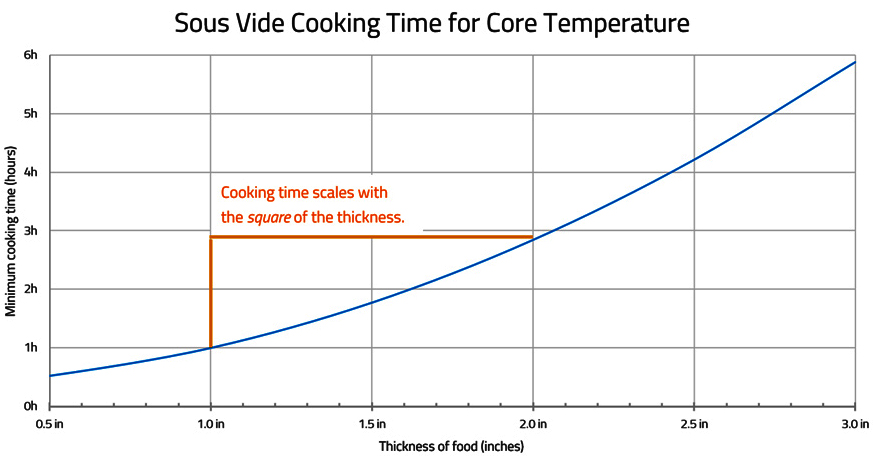
\includegraphics[scale=.5]{sous_vide_plot.jpg}
\end{figure}








\end{document}
